\documentclass[conference,compsoc]{IEEEtran}
\pagestyle{plain}
\usepackage{cite}
\usepackage{amsmath}
\usepackage{amsfonts}
\usepackage{algorithmic}
\usepackage[numbers]{natbib}
\usepackage{lipsum}
\usepackage{multirow, tabularx}
\usepackage{subcaption}
\usepackage[]{footmisc}
\bibliographystyle{IEEEtranN}
\usepackage{graphicx}
% *** GRAPHICS RELATED PACKAGES ***
%
\ifCLASSINFOpdf
  % \usepackage[pdftex]{graphicx}
  % declare the path(s) where your graphic files are
  % \graphicspath{{../pdf/}{../jpeg/}}
  % and their extensions so you won't have to specify these with
  % every instance of \includegraphics
  % \DeclareGraphicsExtensions{.pdf,.jpeg,.png}
\else
  % or other class option (dvipsone, dvipdf, if not using dvips). graphicx
  % will default to the driver specified in the system graphics.cfg if no
  % driver is specified.
  % \usepackage[dvips]{graphicx}
  % declare the path(s) where your graphic files are
  % \graphicspath{{../eps/}}
  % and their extensions so you won't have to specify these with
  % every instance of \includegraphics
  % \DeclareGraphicsExtensions{.eps}
\fi
% graphicx was written by David Carlisle and Sebastian Rahtz. It is
% required if you want graphics, photos, etc. graphicx.sty is already
% installed on most LaTeX systems. The latest version and documentation
% can be obtained at: 
% http://www.ctan.org/pkg/graphicx
% Another good source of documentation is "Using Imported Graphics in
% LaTeX2e" by Keith Reckdahl which can be found at:
% http://www.ctan.org/pkg/epslatex
%
% latex, and pdflatex in dvi mode, support graphics in encapsulated
% postscript (.eps) format. pdflatex in pdf mode supports graphics
% in .pdf, .jpeg, .png and .mps (metapost) formats. Users should ensure
% that all non-photo figures use a vector format (.eps, .pdf, .mps) and
% not a bitmapped formats (.jpeg, .png). The IEEE frowns on bitmapped formats
% which can result in "jaggedy"/blurry rendering of lines and letters as
% well as large increases in file sizes.
%
% You can find documentation about the pdfTeX application at:
% http://www.tug.org/applications/pdftex


% *** ALIGNMENT PACKAGES ***
%
%\usepackage{array}
% Frank Mittelbach's and David Carlisle's array.sty patches and improves
% the standard LaTeX2e array and tabular environments to provide better
% appearance and additional user controls. As the default LaTeX2e table
% generation code is lacking to the point of almost being broken with
% respect to the quality of the end results, all users are strongly
% advised to use an enhanced (at the very least that provided by array.sty)
% set of table tools. array.sty is already installed on most systems. The
% latest version and documentation can be obtained at:
% http://www.ctan.org/pkg/array


% IEEEtran contains the IEEEeqnarray family of commands that can be used to
% generate multiline equations as well as matrices, tables, etc., of high
% quality.



% *** SUBFIGURE PACKAGES ***
%\ifCLASSOPTIONcompsoc
%  \usepackage[caption=false,font=footnotesize,labelfont=sf,textfont=sf]{subfig}
%\else
%  \usepackage[caption=false,font=footnotesize]{subfig}
%\fi
% subfig.sty, written by Steven Douglas Cochran, is the modern replacement
% for subfigure.sty, the latter of which is no longer maintained and is
% incompatible with some LaTeX packages including fixltx2e. However,
% subfig.sty requires and automatically loads Axel Sommerfeldt's caption.sty
% which will override IEEEtran.cls' handling of captions and this will result
% in non-IEEE style figure/table captions. To prevent this problem, be sure
% and invoke subfig.sty's "caption=false" package option (available since
% subfig.sty version 1.3, 2005/06/28) as this is will preserve IEEEtran.cls
% handling of captions.
% Note that the Computer Society format requires a sans serif font rather
% than the serif font used in traditional IEEE formatting and thus the need
% to invoke different subfig.sty package options depending on whether
% compsoc mode has been enabled.
%
% The latest version and documentation of subfig.sty can be obtained at:
% http://www.ctan.org/pkg/subfig




% *** FLOAT PACKAGES ***
%
%\usepackage{fixltx2e}
% fixltx2e, the successor to the earlier fix2col.sty, was written by
% Frank Mittelbach and David Carlisle. This package corrects a few problems
% in the LaTeX2e kernel, the most notable of which is that in current
% LaTeX2e releases, the ordering of single and double column floats is not
% guaranteed to be preserved. Thus, an unpatched LaTeX2e can allow a
% single column figure to be placed prior to an earlier double column
% figure.
% Be aware that LaTeX2e kernels dated 2015 and later have fixltx2e.sty's
% corrections already built into the system in which case a warning will
% be issued if an attempt is made to load fixltx2e.sty as it is no longer
% needed.
% The latest version and documentation can be found at:
% http://www.ctan.org/pkg/fixltx2e


%\usepackage{stfloats}
% stfloats.sty was written by Sigitas Tolusis. This package gives LaTeX2e
% the ability to do double column floats at the bottom of the page as well
% as the top. (e.g., "\begin{figure*}[!b]" is not normally possible in
% LaTeX2e). It also provides a command:
%\fnbelowfloat
% to enable the placement of footnotes below bottom floats (the standard
% LaTeX2e kernel puts them above bottom floats). This is an invasive package
% which rewrites many portions of the LaTeX2e float routines. It may not work
% with other packages that modify the LaTeX2e float routines. The latest
% version and documentation can be obtained at:
% http://www.ctan.org/pkg/stfloats
% Do not use the stfloats baselinefloat ability as the IEEE does not allow
% \baselineskip to stretch. Authors submitting work to the IEEE should note
% that the IEEE rarely uses double column equations and that authors should try
% to avoid such use. Do not be tempted to use the cuted.sty or midfloat.sty
% packages (also by Sigitas Tolusis) as the IEEE does not format its papers in
% such ways.
% Do not attempt to use stfloats with fixltx2e as they are incompatible.
% Instead, use Morten Hogholm'a dblfloatfix which combines the features
% of both fixltx2e and stfloats:
%
% \usepackage{dblfloatfix}
% The latest version can be found at:
% http://www.ctan.org/pkg/dblfloatfix




% *** PDF, URL AND HYPERLINK PACKAGES ***
%
%\usepackage{url}
% url.sty was written by Donald Arseneau. It provides better support for
% handling and breaking URLs. url.sty is already installed on most LaTeX
% systems. The latest version and documentation can be obtained at:
% http://www.ctan.org/pkg/url
% Basically, \url{my_url_here}.


\begin{document}
\title{A Combination between Genetic Algorithm and Heuristic Algorithm\\ in Electric Vehicle Routing Problem\footnote[1]{This is our final project for CS106 - Artificial Intelligence, University of Information Technology, Vietnam National University, Ho Chi Minh City}}


% author names and affiliations
% use a multiple column layout for up to three different
% affiliations
\author{\IEEEauthorblockN{An Vo, Tan Ngoc Pham}
\IEEEauthorblockA{University of Information Technology,\\ 
Vietnam National University HCMC\\
Email: $\{19520007, 19520925\}$@gm.uit.edu.vn}
}
\maketitle

% As a general rule, do not put math, special symbols or citations
% in the abstract
\begin{abstract}
Driven by the badly directing in the present environment, it is urgent to find out alternative way to reduce the greenhouse gas and using electric vehicles is by far the best choice nowadays. And solving the problem of optimizing routes for the electric vehicles or also known as the Electric Vehicle Routing Problem is considered as a needed problem to be solved. In this paper, we give out a combination between Genetic Algorithm and a simple heuristic for Charging Stations Placement to solve this problem. We divided our problem into two separate sections, which are Electric Vehicle Routing and Locations of Charging Stations.
\begin{IEEEkeywords}
Electric Vehicles, K-means, Heuristics, Distance Optimizing, Genetic Algorithm, Charging Stations Placement
\end{IEEEkeywords}
\end{abstract}

%Introduction
\IEEEpeerreviewmaketitle
\section{Introduction}In present days, the market has a more tendency to compete to each other. The existence for an effective, feasible and environmental-friendly transporting system is a crucial factor of a logistic company. One of the present strategy of those companies is to shift to a newer type of vehicles: Electric Vehicles (EVs). This is understandable due to the continuously raising need for energy alternatives, which is comprehensible due to the present global warming, pollution and climate changes. The problem is such urgent that there are quite a few logistic companies around the world now establish their own campaigns to manufacture CO$_2$-emission reduction of daily operations, e.g. Tesla, FedEx. Among the contributing factor to environmental harm, there is no doubt that transportation is the primary component, which gives out 29\% of the total greenhouse gas emission to the Earth \cite{transportation}. The most effective way to reduce the greenhouse gas, hence, is to use electric vehicles (EVs).\\

The \textit{vehicle routing problem} (VRP) is not a new problem, it was first introduced in 2002 \cite{vrp}. The problem is demonstrated as finding the shortest routing solution for a set of vehicles to visit a set of locations satisfying customers' needs \cite{vrp_demonstration}. Due to the effective of the VRP, there is a wide range of variation to the original problem itself. One of the upgraded versions for VRP is known as the VRP with EVs or the \textit{electric vehicle routing problem} (EVRP) \cite{evrp}, EVRP is considered as a more difficult problem in comparison with the original one due to the recharging decision-making and more complex objective function requiring to minimize distance cost \cite{evrp_difficulties}. EVRP is found to be quite difficult since it is relevant to distribute logistics in not only identifying customers set with a fixed demand but satisfying EVs' energy capacity also. In addition, the ultimate goal is to minimize the total distance between the EVs. And in this paper, we did make a minor change - which is discussed further in 2.1 - to the indigenous version.\\

\textit{Genetic algorithm} (GA) \cite{GA} is a search-based technique which have been used in optimization fields for practical problems. The idea behind the algorithm itself is based on the natural selection given by Charles Darwin's evolutionary synthesis in the 1860s. The basic concept for GA can be understood as the well-performed result will still remain in the population and produce their better successor continuously, while the worse performance is removed. And the process proceeds on and on until the inappropriate individuals become extincted eventually.\\

The rest of this paper is organized as follows. We will discuss some of related work sharing the similarity to our paper in section 2. We also discuss further about mathematical view for EVRP in section 3. Next, section 4 describes about our methods to solve this problem. Then, section 5 will display our results in using methods in the previous section. After that, section 6 will talk more about our limitations and ways to minimize them in our future work. Finally, we will have our final conclusion for the whole paper.

\section{Related work}
Solving the EVRP with an effective solution is an urgent need, and it is clear to realize in the study below. Throughout this work, we solve the electric vehicle routing and location of Charging Stations (CSs) separately. The mentioned research, thus, is divided into two individual sections.

\subsection{Location of charging stations}
Location of CSs is a problem with multiple objective functions, e.g. energy cost and total travel distance.\\

\citeauthor{locationCS} (\citeyear{locationCS}) \cite{locationCS} proposed a GA for location of CSs considering actual demand of electric energy consumption, with different capacities and energy levels between vehicles. \citeauthor{locationCS2} (\citeyear{locationCS2}) \cite{locationCS2} proposed a two-phases solution. In the first one, they use K-means \cite{k-means} to divide the market into regions based on demands. They use a model to acknowledge locations of CSs while still maximizing operational productivity in the second one.\\

\citeauthor{locationCS3} (\citeyear{locationCS3}) \cite{locationCS3} proposed a mathematical formulation for the problem and they provide four strategies to solve that problem, including mixed integer linear programming iterative method, greedy algorithm, mixed integer linear programming approach, chemical reaction optimization. \citeauthor{locationCS4} (\citeyear{locationCS4}) \cite{locationCS4} also proposed four solution strategies for the location of CSs and a heuristic solution for electric vehicle routing. Comparing to other strategies, K-means gives out the best performance when locating the charging stations at the centroid of the cluster.\\

\citeauthor{locationCS5} (\citeyear{locationCS5}) \cite{locationCS5} proposed a effective genetic algorithm with crossover, mutation and initialization. Hence, GA's operations in this work is mostly based on the forementioned paper. This paper, however, goes through all the charging stations once only. \citeauthor{locationCS6} (\citeyear{locationCS6}) \cite{locationCS6} proposed an efficient branch and cut framework and a three-phase heuristic algorithm that can efficiently solve a variety of instances for min-max electric vehicle routing problem (MEVRP). They use a wide range of techniques, e.g. Variable Neighborhood Search, LKH Heuristic, Genetic Algorithm.\\

Almost recent studies show the advance in researching for this problem. Late trends are to propose modelizing the problem into mathematical formulas, as well as differently problem-approaching strategies. And among those highlighted K-means strategy, which seems to be quite simple but highly effective.

\subsection{Electric vehicle routing}
At the beginning, the Electric Vehicle Routing problem was invariant and far different from what we know nowadays \cite{evr0}.\\

The vehicle routing problem was first laid the ground by \citeauthor{evr} in \citeyear{evr} \cite{evr}; they showed the explanation for the problem of assigning stations for vehicles to travel between two any given points in the shortest way and satisfy all the customers' demands. And five years later, the problem was formalised and mathematically demonstrated for both computer solving and human solving by \citeauthor{evr2} in \citeyear{evr2} \cite{evr2}.\\

\citeauthor{evr3} (\citeyear{evr3}) \cite{evr3} showed the importance and potential for the vehicle routing problem in our present $21^{st}$ days by manifesting its variants and differently approaching techniques from 2009 to 2015; and Metaheuristic algorithms by far outweighed the others. There, one of the most investigated variants for the VRP was the EVRP due to the need for cost reducing and protecting the environment in the industry. The solution for the problem was also first proposed as in \citeauthor{evr3} after considering several restrictions.\\

The exact problem of the EVRP with recharging stations and an exact method was first introduced by \citeauthor{evr4} (\citeyear{evr4}) \cite{evr4}. In this work, the author gave a exact demonstration for a sub-problem in the present EVRP nowadays of which EVs are enabled to recharging battery after traveling at customers nodes. In later times, \citeauthor{evr5} (\citeyear{evr5}) \cite{evr5} proposed two construction heuristics, which are the Modified Clarke - Wright Savings heuristic and the Density-Based Clustering Algorithm, was shown to work efficiently on the problem of Green Vehicle Routing Problem (GVRP). \citeauthor{evr6} (\citeyear{evr6}) \cite{evr6} proposed a mathematical formulation to modelize multiple constraints in the Electric Vehicle Routing Problem with Time Windows (EVRP-TW).\\

Reviewing these proposals and approaching point to solve the EVRP, we might consider to use heuristics and metaheuristics instead of exact strategies. This is comprehensible due to the unpredictable customers' demands and too many constraints for an exact efficient solution strategy to handle.

%Problem statement
\section{Problem statement}
The EVRP is an extension of the original NP-hard VRP problem, of which goal is to find the smallest route for all vehicles to satisfy all customers' demands, and with the constraint of starting and ending at the central depot. The additional constraint for the EVRP is that there are battery charge level limits and recharging decision-making.\\

The mathematical model of the EVRP is a fully connected weighted graph $G(V, A)$, where $V = U \cup R$ such that $U = \{1,...,n\}$  is a set of $n$ nodes (customers) in the graph, $R = \{n + 1,...,n + s\}$ is a set of $s$ recharging stations for EVs, set $F'$ denotes the set of $R$ recharging station, a central depot $0$ as the starting point for all EVs, and $A = \{\left(i, j\right)\text{ }|\text{ } i, j \in N, i \neq j\}$ is a set of arcs connecting those nodes.\\

For every arc in the graph, it is assigned to a non-negative real value $d_{ij} \in \mathbb{R}^+$ as the Euclidean distance between two connected nodes $i$ and $j$ and for every node $i$ labeled as customer has a positive demand $b_i \in U$. Besides, each EV traveling in the arc $\left(i, j\right)$ will consume an energy amount $\rho d_{ij}$, in which $\rho$ is a constant denoting the consumption rate for all EVs.\\

The solution for the EVRP is modelized as an objective function $\phi$, then our task is to find a set of routes satisfying all the customers' demand, having the minimum total traveling time, followed by the conditions as:
\begin{itemize}
    \item EVs all start (with a full energy level and full load) and end at the central depot.
    \item All recharging stations should be visited multiple times on the go. (central depot included).
    \item Customer nodes are visited only once by one EV.
    \item The total demand of customers does not exceed the EV's total capacity $C$ for every single route.
    \item The total energy consumption must not exceed any maximal battery charge level $Q$ for every single route.
    \item EVs leave the charging station with a full battery charge level.
\end{itemize}
Mathematically, the EVRP is expressed as \cite{evrp_benchmark}:

%1
\begin{equation}
    \min \phi = \sum_{\left(i, j \in U \cup R\right) \land \left(i \neq j \right)}{d_{ij}x_{ij}}
\end{equation}
s.t.

%2
\begin{equation}
    \sum_{\forall i \in U \cup R, j \in V, i \neq j}{x_{ij}} = 1
\end{equation}
where two these equations respectively define the EVRP objective function and enforce the connectivity of customer visits.\\
%3
\begin{equation}
    \sum_{j \in V, i \neq j}{x_{ij}} \leq 1, \forall i \in F'
\end{equation}
The third equation handles the connectivity of recharging stations.\\
%4
\begin{equation}
    \sum_{j \in V, i \neq j}{x_{ij}} - \sum_{j \in V, i \neq j}{x_{ji} = 0, \forall i \in V}
\end{equation}
Equation (4) establishes flow conservation, i.e., by assuring that for every node, the number of incoming arcs is equal to the number of outgoing ones.\\
%5
\begin{equation}
    u_j \leq u_i - b_ix_{ij} + C\left(1-x_{ij}\right), \forall i\in V, \forall j \in V, i \neq j
\end{equation}
%6
\begin{equation}
    0 \leq u_i \leq C, \forall i \in V
\end{equation}
s.t. variables $u_i$ denote the remaining carrying capacity of an EV on its arrival at node $i \in V$. Equations (5) and (6) are to assure all customers' demands are all fulfilled via a non-negative carrying load upon arrival at any node (the depot included).\\
%7
\begin{equation}
    y_j \leq y_i -\rho d_{ij}x_{ij}, \forall i \in I, \forall j \in V, i \neq j
\end{equation}

%8
\begin{equation}
    y_j \leq Q-\rho d_{ij}x_{ij}, \forall i \in F' \cup \{0\}, \forall j \in V, i \neq j
\end{equation}

%9
\begin{equation}
    0 \leq y_i \leq Q, \forall i \in V
\end{equation}
where variable $y_i$ denotes the remaining battery charge level of an EV on its arrival at node $i \in V$. The condition that the battery charge never falls below 0 is guaranteed by equations (7), (8) and (9).\\
%10
\begin{equation}
    x_{ij} \in \{0,1\}, \forall i \in V, \forall j \in V, i \neq j
\end{equation}
The last equation defines a set of binary decision variables to recognized whether an arc is traveled or not valued by 1 and 0 respectively. 

\section{Methods}
This method is inspired by \citeauthor{evrptw} (\citeyear{evrptw}) \cite{evrptw}. Since the Electric Vehicle Routing Problem is a NP-hard problem with sophisticated constraints, there is no obvious optimal solution to the problem itself, thus we have to approximate the solution as optimal as possible. In this paper, Genetic Algorithm is proposed as a promising solution to solve the EVRP.\\

The problem is encoded in such a way that the depot (0), customer nodes (1,...,n) and recharging stations (n + 1, n + 2,...,n +m) are encoded by a natural number, and the gene values are put into order of visiting sequence \cite{evrptw}. Figure 1 demonstrates the way three routes of 3 EVs are encoded into a chromosome: EV 1 starts from the depot 0 and visits customer node 5 and 3 and returns to the depot after recharging at recharging nodes 6 and visits customer node 7; EV 2 from the depot travels to customer node 8 and recharges at recharging node 9, then it visits customer node 2 and returns to the depot; EV 3 starts from the depot, visits customer nodes 4, 1 and 10 and returns to the depot without a need to recharge.

\begin{figure}[h!]
    \centering
    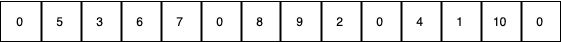
\includegraphics[scale=0.42]{1}
    \caption{Chromosome representation of a problem}
    \label{fig:my_label}
\end{figure}


GA's procedure is divided into 5 separate steps, which are:\\

\textit{Initialization}: In this step, we randomly assign the code number for customer nodes in the genes, but we do not execute the same thing for Recharging Stations. In order to generate a better population, we use \textit{K-means} \cite{k-means} to initialize chromosomes (individual): we choose $k = $ number of EV in the problem, and for every gene in our population, we will choose a different random seed to guarantee the diversity of the original population. We have to ensure that the population involves $N$ individuals, s.t. $N = $ number of customers $+$ number of EV $+$ 1, the initialization satisfy the customer needs for each node and never do an EV exceed the loading capacity $Q$ as well.\\ Let denote $q_i'$ as the customer node's demand. We shall add number 0 after the $t$ gene in the chromosome if $\sum_{i = 1}^{t}{q'_i \leq Q}$ and $\sum_{i = 1}^{t+1}{q'_i < Q}$. We will repeatedly execute this number $0$ insertion $n - 1$ times in both first and last gene respectively.\\

\textit{Evaluation}: In this paper, we will use fitness value $f(i) = \sum_{\left(i, j \in U \cup R\right) \land \left(i \neq j \right)}{d_{ij}x_{ij}}$. The smaller our fitness value, the better our solution quality. On the contrary, the fitness value is invalid when $f(i) = \infty$. An invalid solution is when the constraint of the EVs' capacity or the EVs' energy capacity is violated. However, we realized that violating the EVs' capacity constraint is much worse than violating the energy one. This is because we can fix the energy capacity constraint by improving our heuristic function for charging stations placement, but in other hands, capacity violating makes our solution meaningless.\\


\textit{Selection}: In this problem, we choose the \textit{Tournament Selection} \cite{tournament-selection} as the key. Tournament Selection is a method to choose an individual from a population of individuals in a Genetic Algorithm. It consists of several tournaments between a few randomly chosen individuals from the population. The winner (individual with the best fitness) in each tournament is selected to proceed the crossover process. \\

\textit{Heuristic function to add recharging stations}: We create an energy list $e$, in which $e_i$ is the distance from node $i$ to the nearest charging station, at the beginning. Then, we will loop through each element $i$ in the population's individual, if the sum of total energy consumption from beginning to node $i$ and sufficient energy to get to the next node (node $i + 1$) is larger than $Q$ subtracted by $e_{i + 1}$, after that we will add the charging stations between node $i$ and node $i + 1$ via Dijkstra algorithm \cite{dijkstra}, in which the starting point is node $i$, the ending point is node $i + 1$ and the rest in graph is charging stations. We only add the edges between two vertices into graph if energy cost of those does not exceed the EV's remaining energy.\\
The result of Dijkstra algorithm is a list of charging stations and we will add these nodes into between node $i$ and $i+1$ in this individual.\\

\textit{Crossover}: We realized that keeping charging stations in individuals will make the problem more difficult when individual's size is not the same in the population. Furthermore, recharging stations do not play an important role when it comes to crossover process. We will get rid of all existing recharging stations from the whole population in this step, thus.\\
The crossover procedure consists of 6 sub-steps:
\begin{enumerate}
    \item Remove all recharging stations in the population.
    
    \item Randomly choose a segment of genes in the chromosome.
    \begin{figure}[h!]
    \centering
    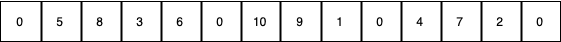
\includegraphics[scale=0.42]{2}
    \caption{Randomly choose the sub-solution in parents 1}
    \label{fig:my_label}
\end{figure}

    \begin{figure}[h!]
    \centering
    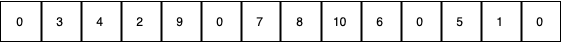
\includegraphics[scale=0.42]{3}
    \caption{Randomly choose the sub-solution in parents 2}
    \label{fig:my_label}
\end{figure}

    \item Move the selected sub-path in each parent to the front genes in the chromosome.
    
    \begin{figure}[h!]
    \centering
    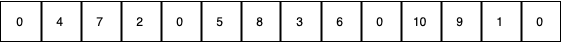
\includegraphics[scale=0.42]{4}
    \caption{Change the sub-solution in parents 1 to the front}
    \label{fig:my_label}
\end{figure}

    \begin{figure}[h!]
    \centering
    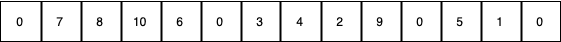
\includegraphics[scale=0.42]{5}
    \caption{Change the sub-solution in parents 2 to the front}
    \label{fig:my_label}
\end{figure}


    \item Keep sub-path of the first chromosome in offspring 1, add the genes of the second chromosome which the first chromosome does not include after sub-path as their sequence. Add number 0 in the last gene of chromosome.
    
    \begin{figure}[h!]
    \centering
    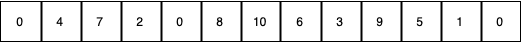
\includegraphics[scale=0.42]{7}
    \caption{Offspring 1}
    \label{fig:my_label}
\end{figure}
    
    \begin{figure}[h!]
    \centering
    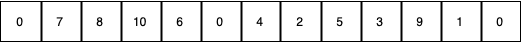
\includegraphics[scale=0.42]{8}
    \caption{Offspring 2}
    \label{fig:my_label}
\end{figure}

    \item Add number 0 in any gene after the first sub-path and select the offspring with the highest value of fitness. The second offspring is obtained in the same manner.
     \begin{figure}[h!]
    \centering
    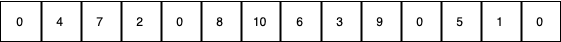
\includegraphics[scale=0.42]{9}
    \caption{Add number 0 to any genes randomly}
    \label{fig:my_label}
\end{figure}

    \begin{figure}[h!]
    \centering
    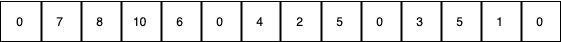
\includegraphics[scale=0.42]{10}
    \caption{Add number 0 to any genes randomly}
    \label{fig:my_label}
\end{figure}
    \item Add recharging stations to every chromosome in the population.\\
    
\end{enumerate}

\textit{Mutation}: Although GA requires mutation step, we do not use this step in our paper.\\

\textit{Terminated criterion}: We will stop the procedure once the number of iteration exceeds the maximum value or our population converges, which means all the individuals are perfectly identical. Or else, if both conditions are not satisfied, we will return and continue the above process.\\
\newpage
\newpage

\begin{figure}[h!]
    \centering
    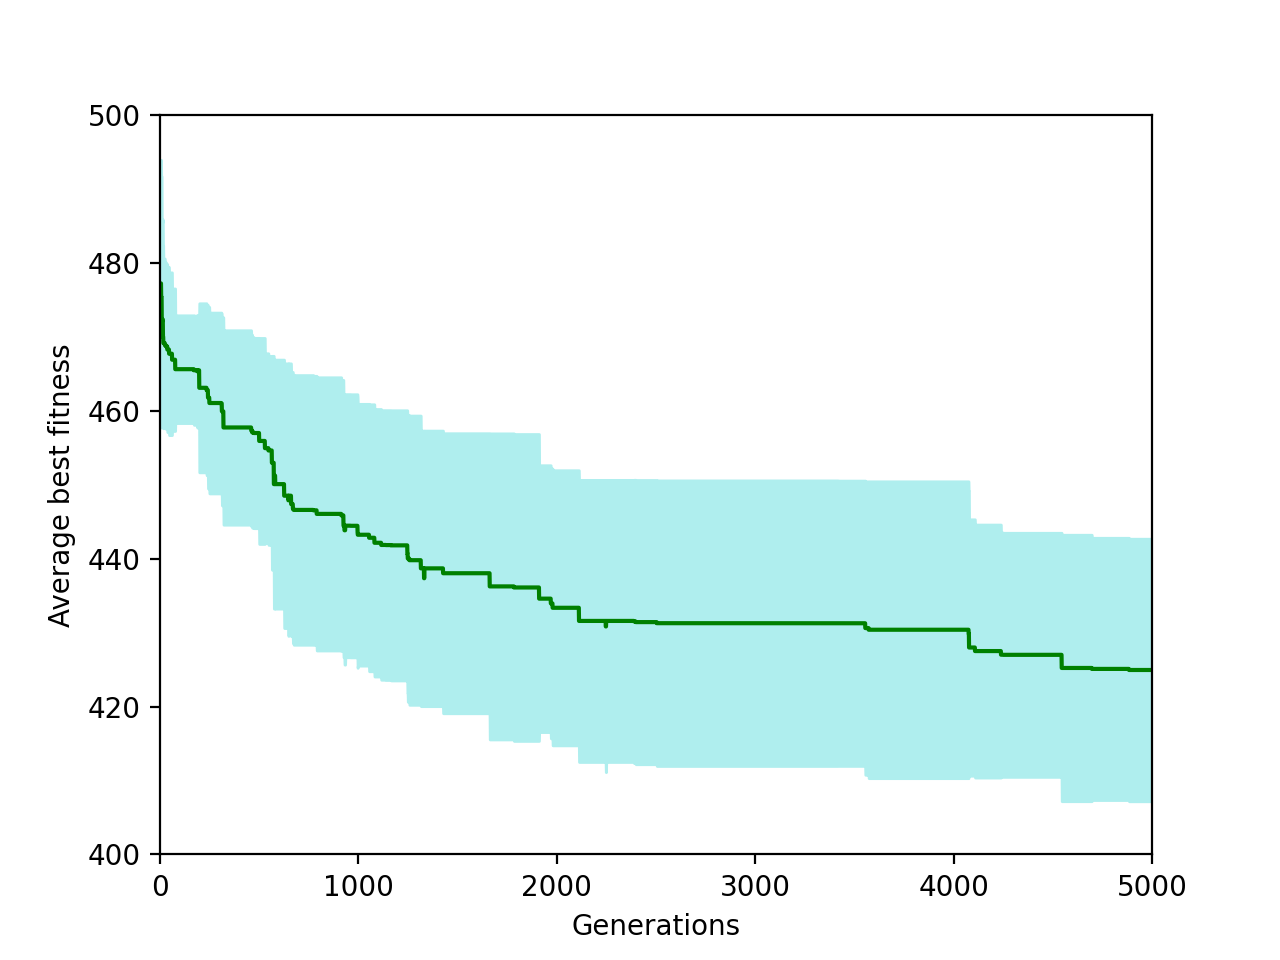
\includegraphics[scale=0.35]{E-n22-k4}
    \caption{E-n22-k4}
    \label{fig:my_label}
\end{figure}

\begin{figure}[h!]
    \centering
    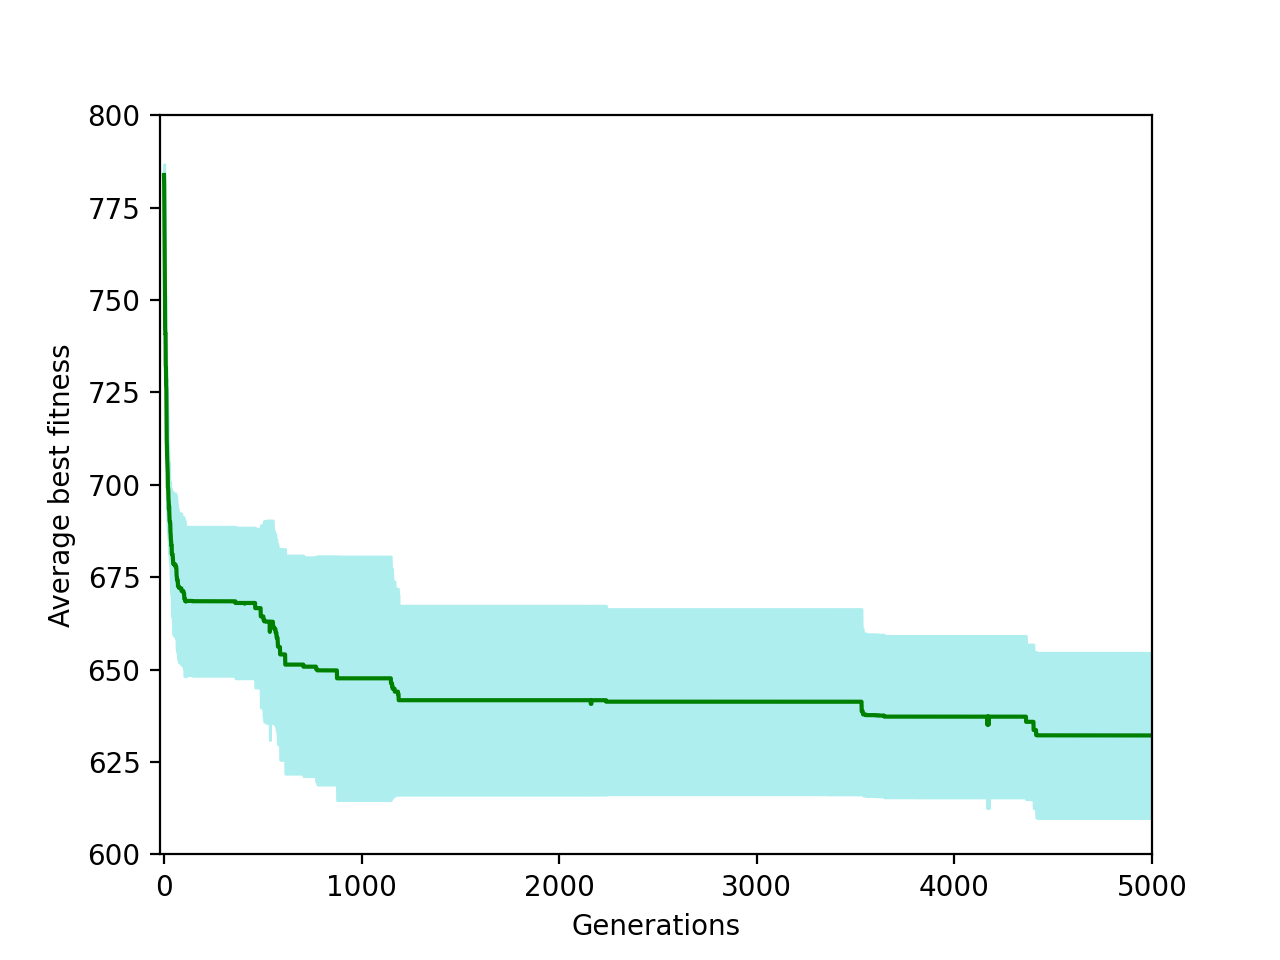
\includegraphics[scale=0.35]{E-n23-k3}
    \caption{E-n23-k3}
    \label{fig:my_label}
\end{figure}

\begin{figure}[h!]
    \centering
    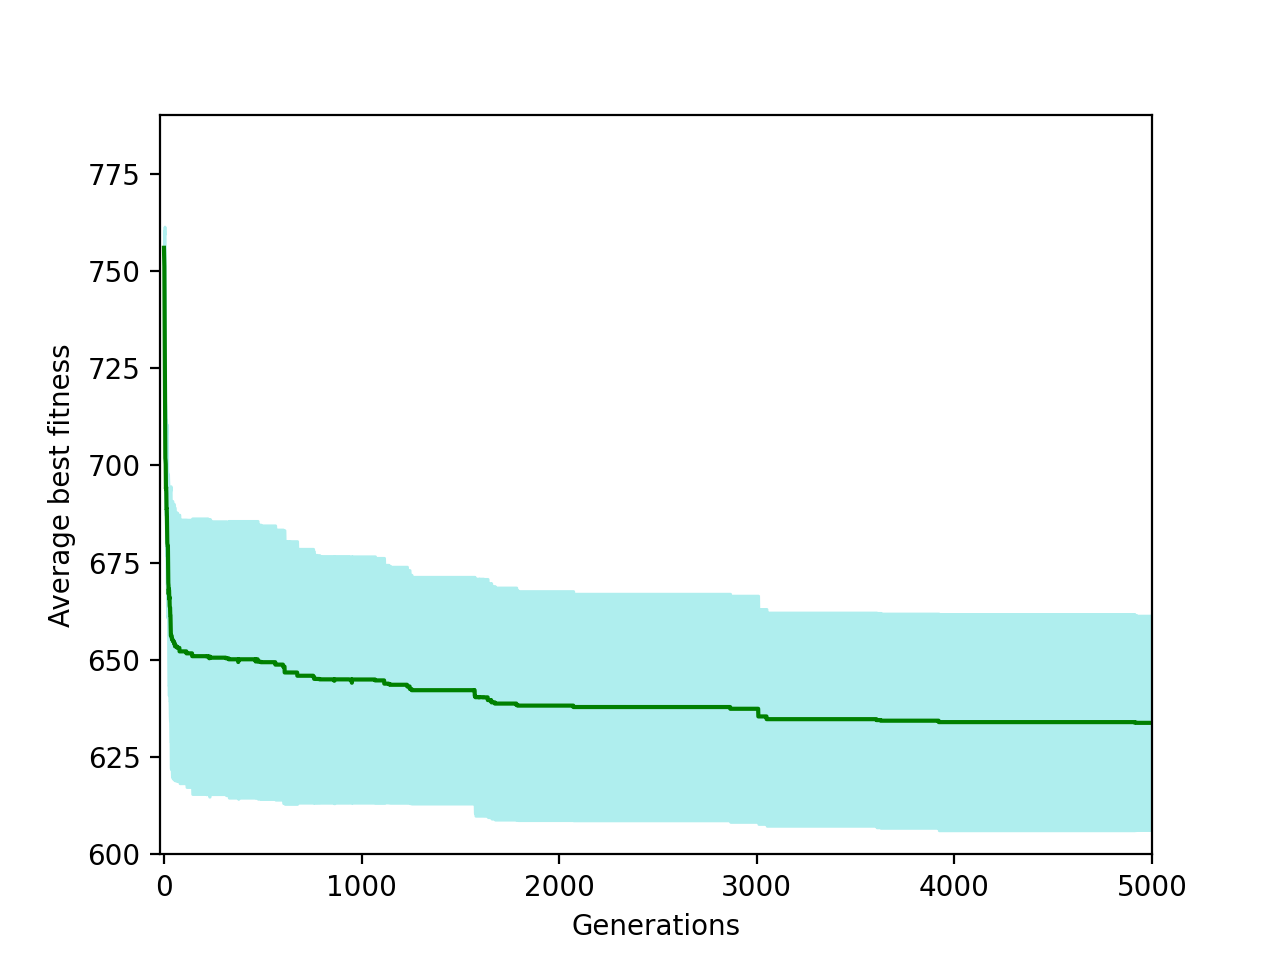
\includegraphics[scale=0.35]{E-n30-k3}
    \caption{E-n30-k3}
    \label{fig:my_label}
\end{figure}

\begin{figure}[h!]
    \centering
    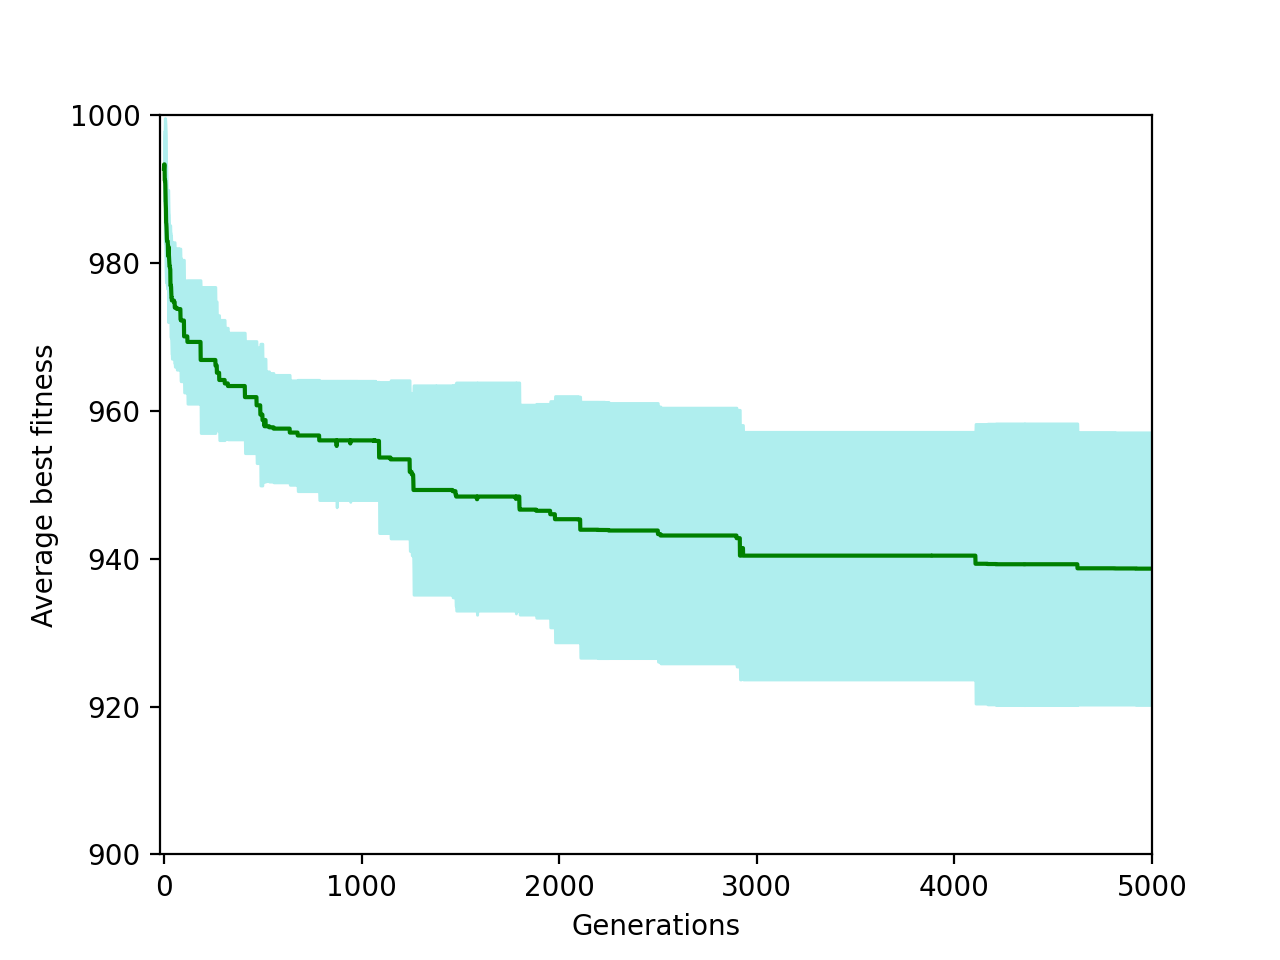
\includegraphics[scale=0.35]{E-n33-k4}
    \caption{E-n33-k4}
    \label{fig:my_label}
\end{figure}
\newpage
\begin{figure}[h!]
    \centering
    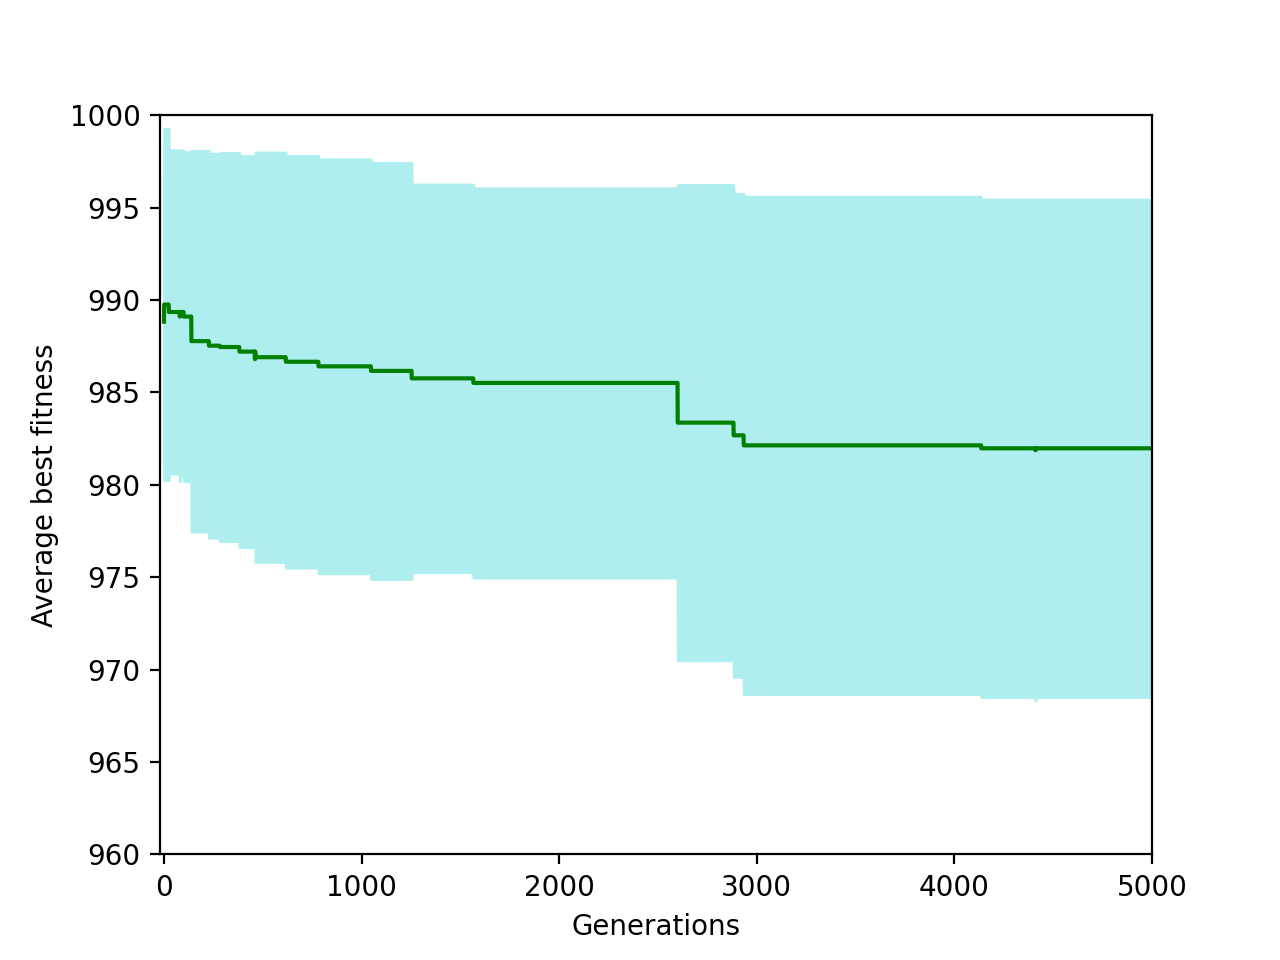
\includegraphics[scale=0.35]{E-n51-k5}
    \caption{E-n51-k5}
    \label{fig:my_label}
\end{figure}

\begin{figure}[h!]
    \centering
    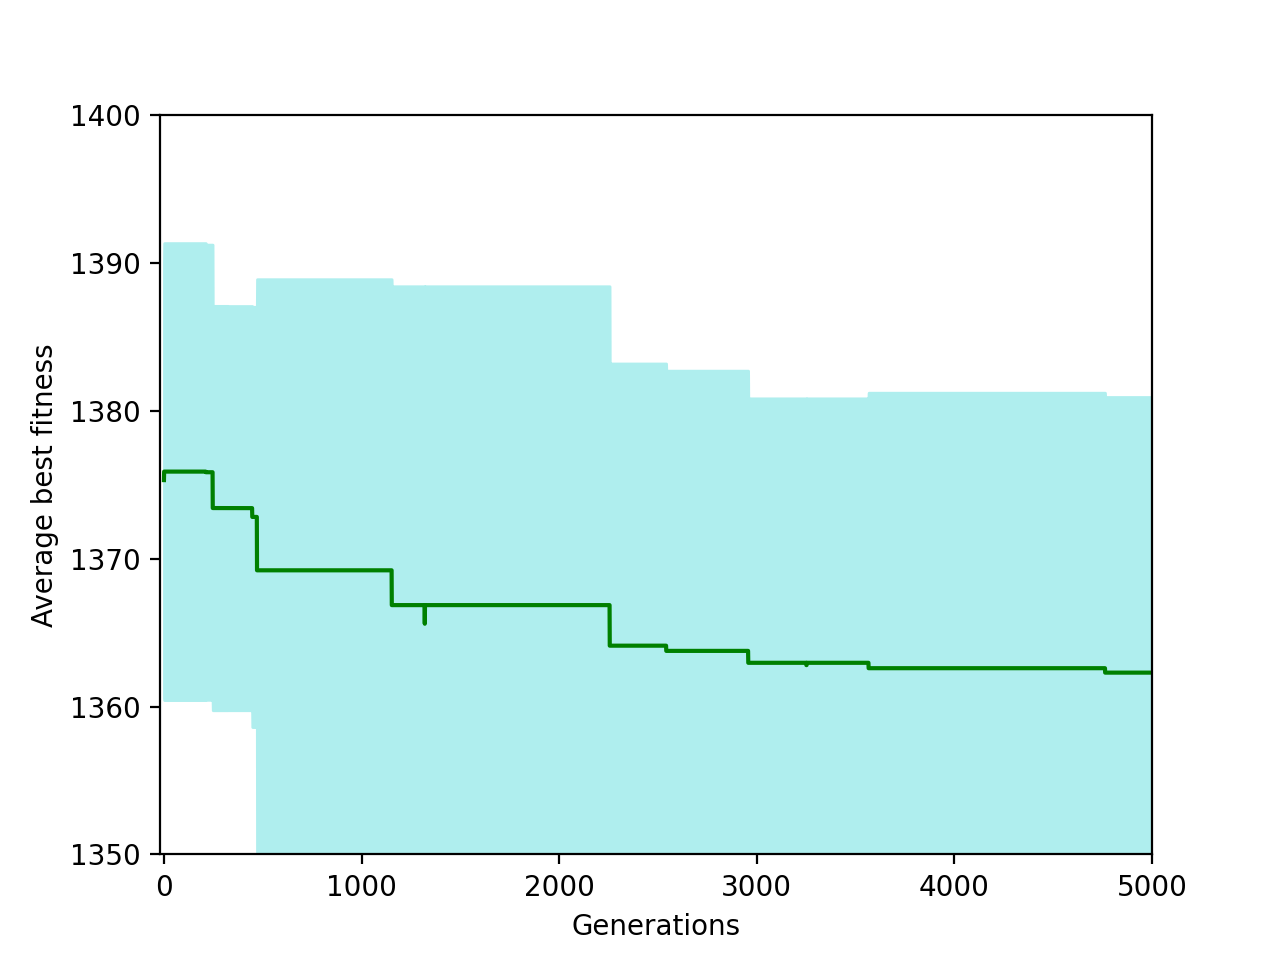
\includegraphics[scale=0.35]{E-n76-k7}
    \caption{E-n76-k7}
    \label{fig:my_label}
\end{figure}


\begin{figure}[h!]
    \centering
    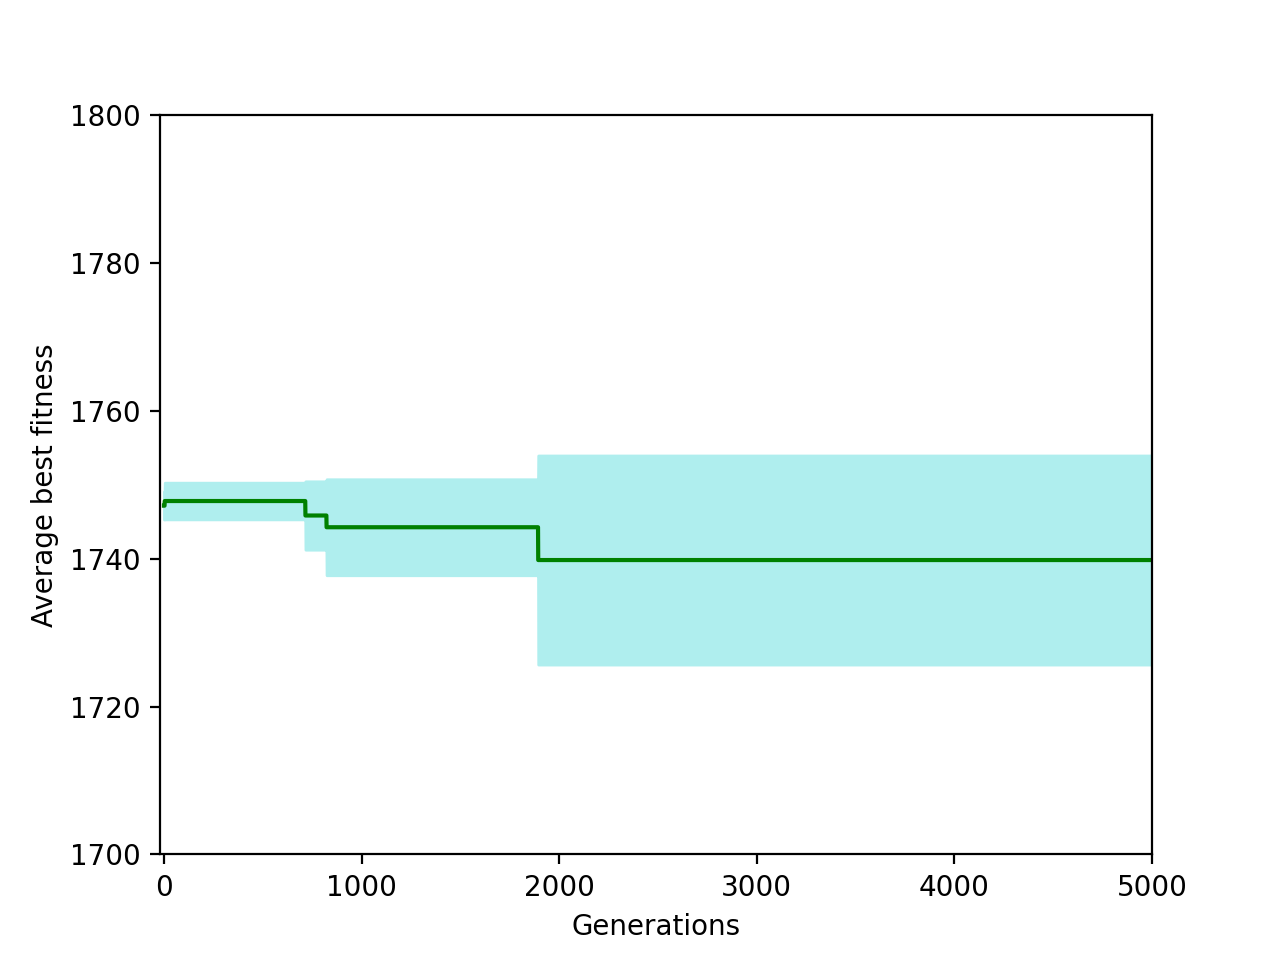
\includegraphics[scale=0.35]{E-n101-k8}
    \caption{E-n101-k8}
    \label{fig:my_label}
\end{figure}


\begin{figure}[h!]
    \centering
    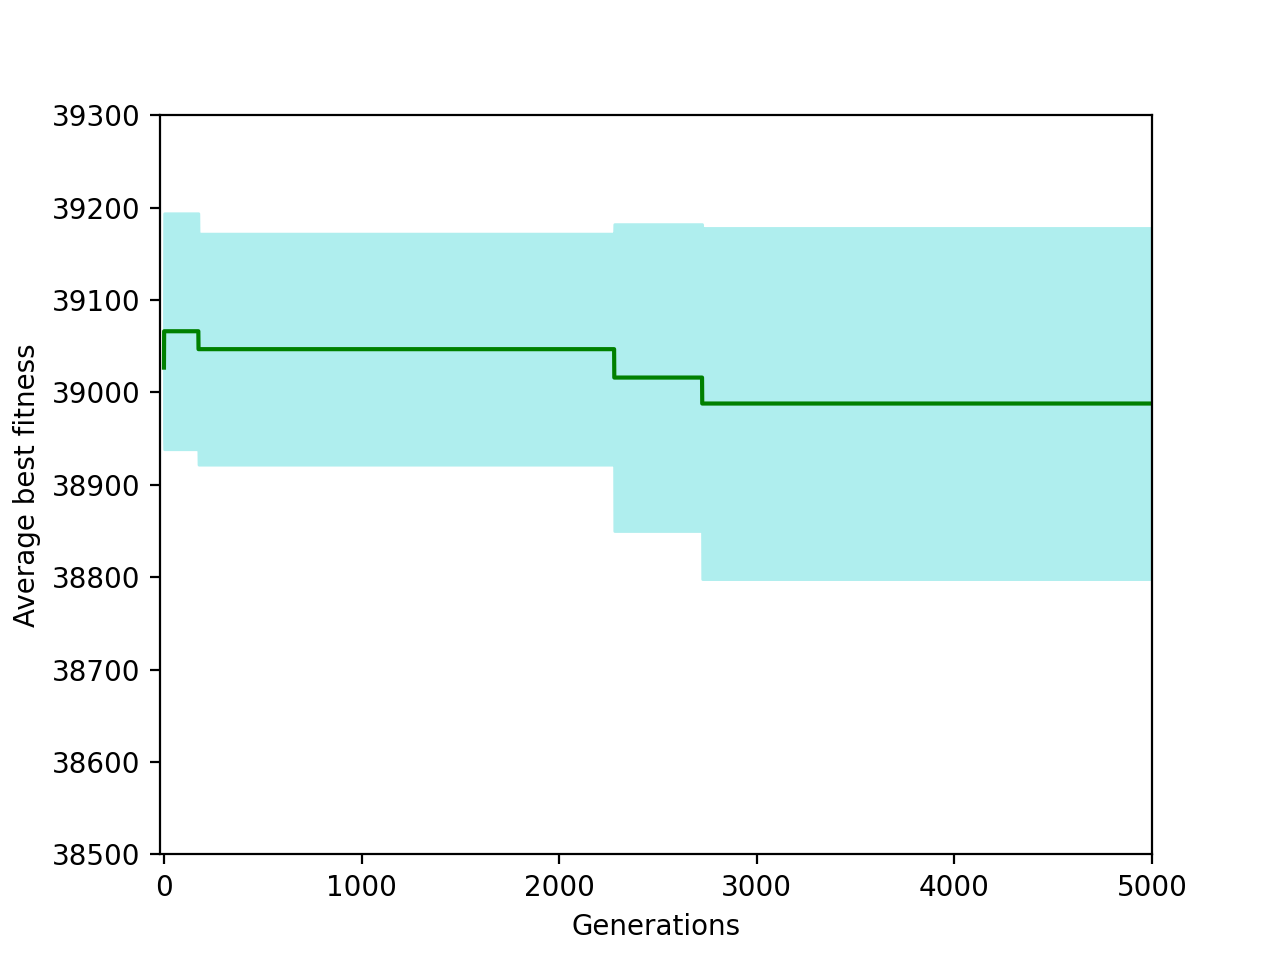
\includegraphics[scale=0.35]{X-n143-k7}
    \caption{X-n143-k7}
    \label{fig:my_label}
\end{figure}
\newpage

\begin{figure}[h!]
    \centering
    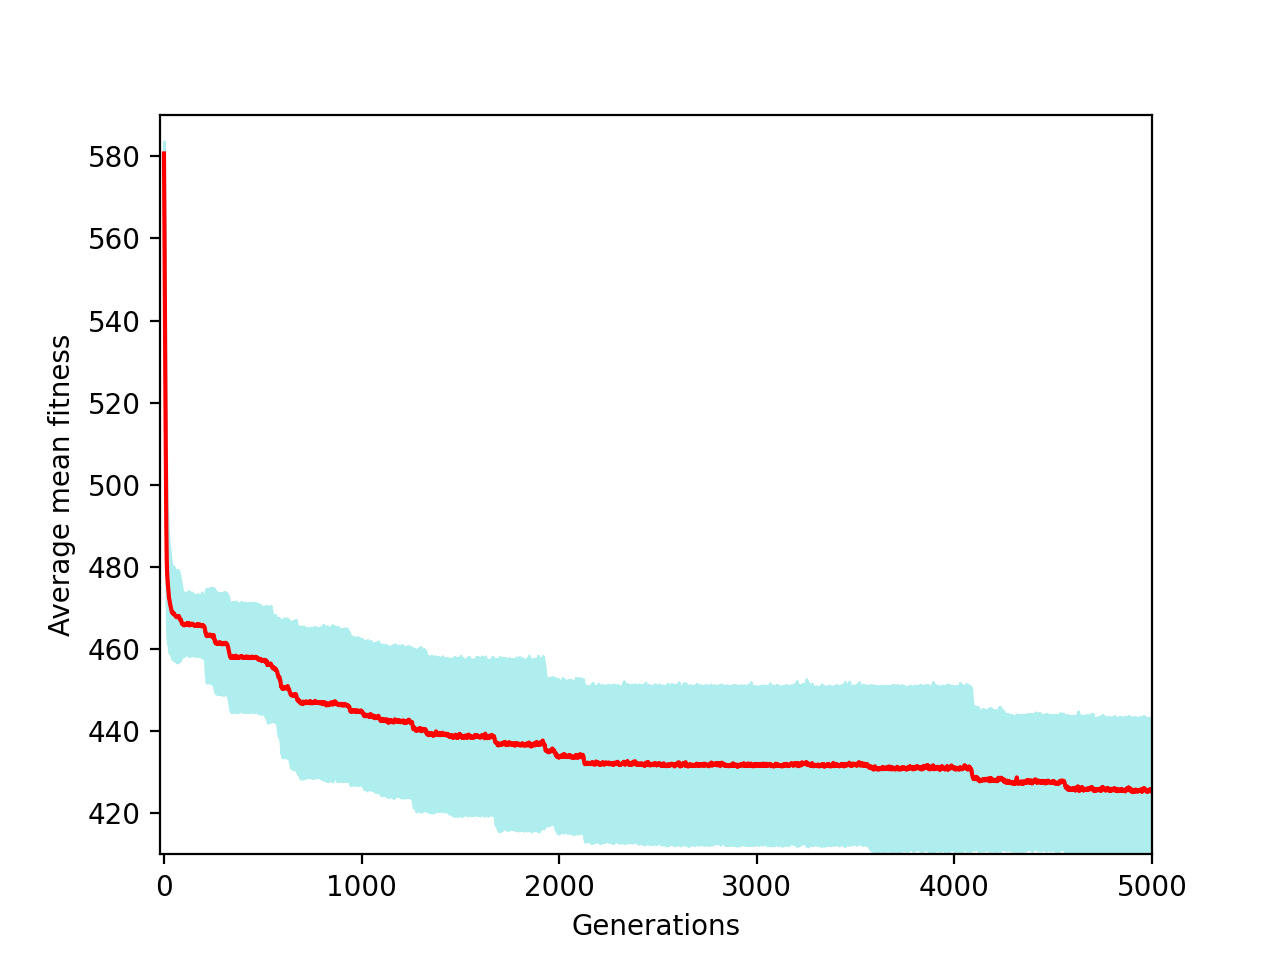
\includegraphics[scale=0.35]{E-n22-k4-mean}
    \caption{E-n22-k4}
    \label{fig:my_label}
\end{figure}

\begin{figure}[h!]
    \centering
    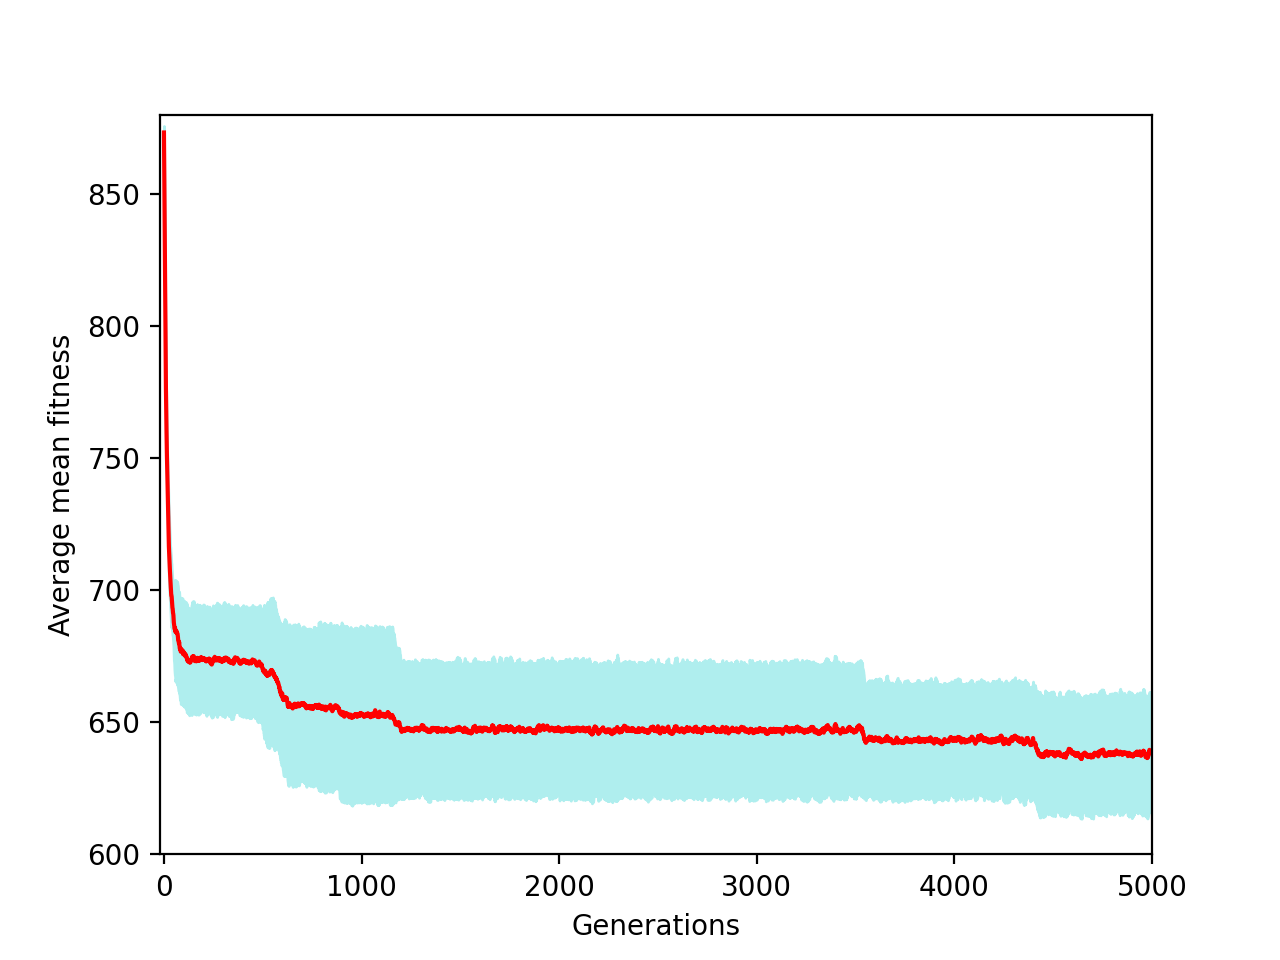
\includegraphics[scale=0.35]{E-n23-k3-mean}
    \caption{E-n23-k3}
    \label{fig:my_label}
\end{figure}

\begin{figure}[h!]
    \centering
    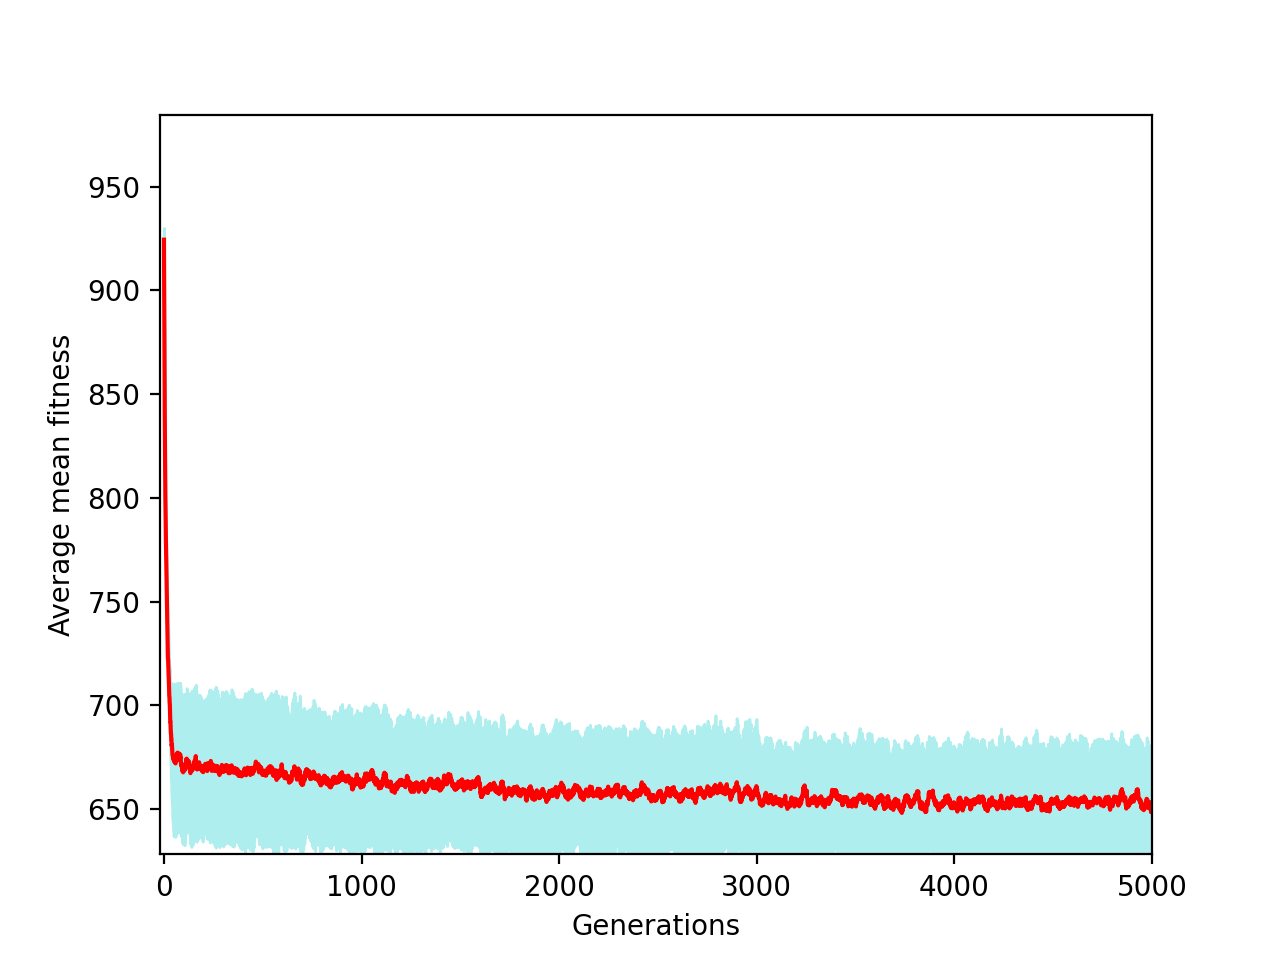
\includegraphics[scale=0.35]{E-n30-k3-mean}
    \caption{E-n30-k3}
    \label{fig:my_label}
\end{figure}

\begin{figure}[h!]
    \centering
    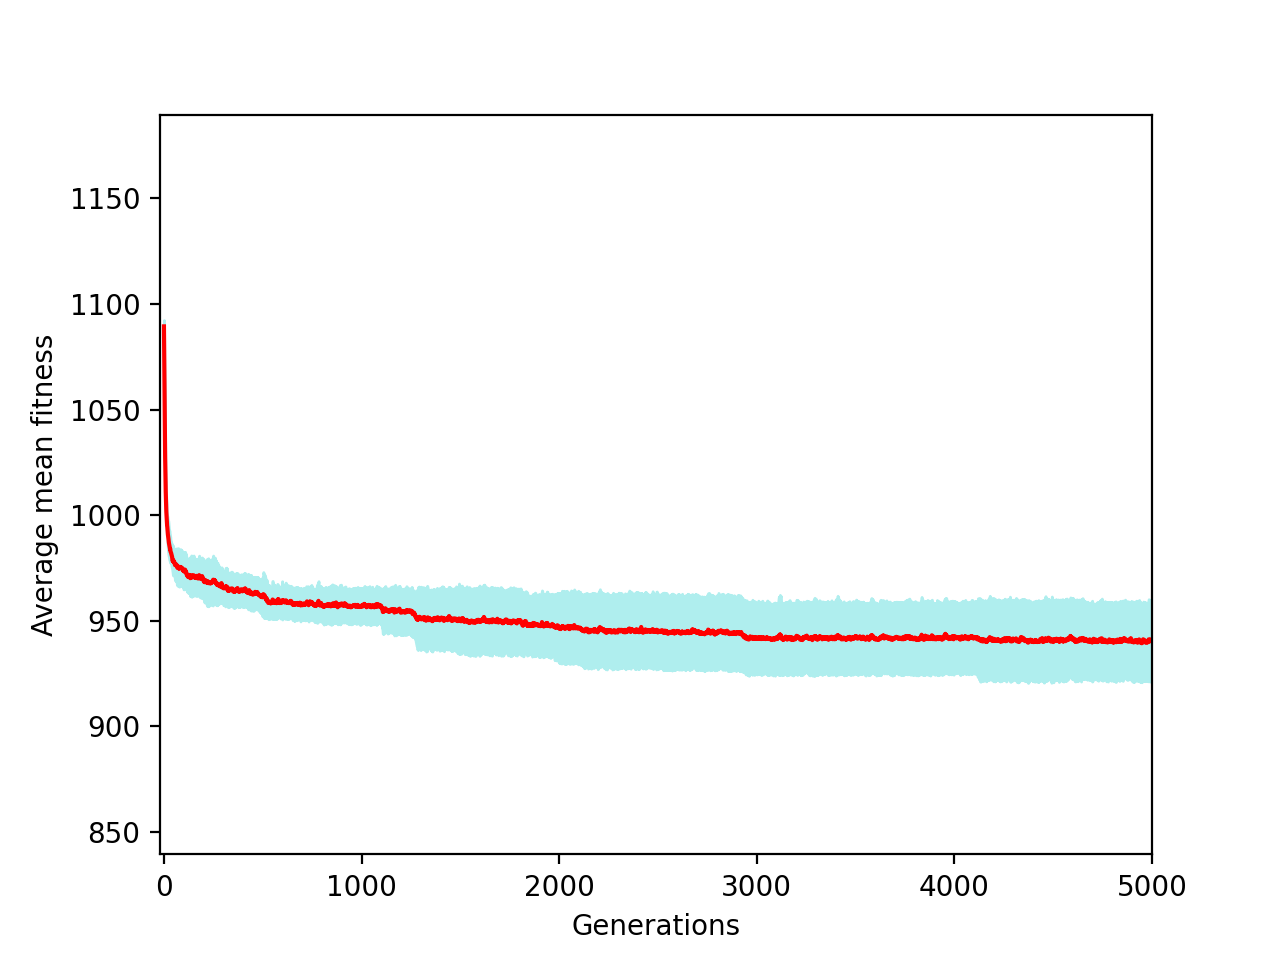
\includegraphics[scale=0.35]{E-n33-k4-mean}
    \caption{E-n33-k4}
    \label{fig:my_label}
\end{figure}
\newpage
\begin{figure}[h!]
    \centering
    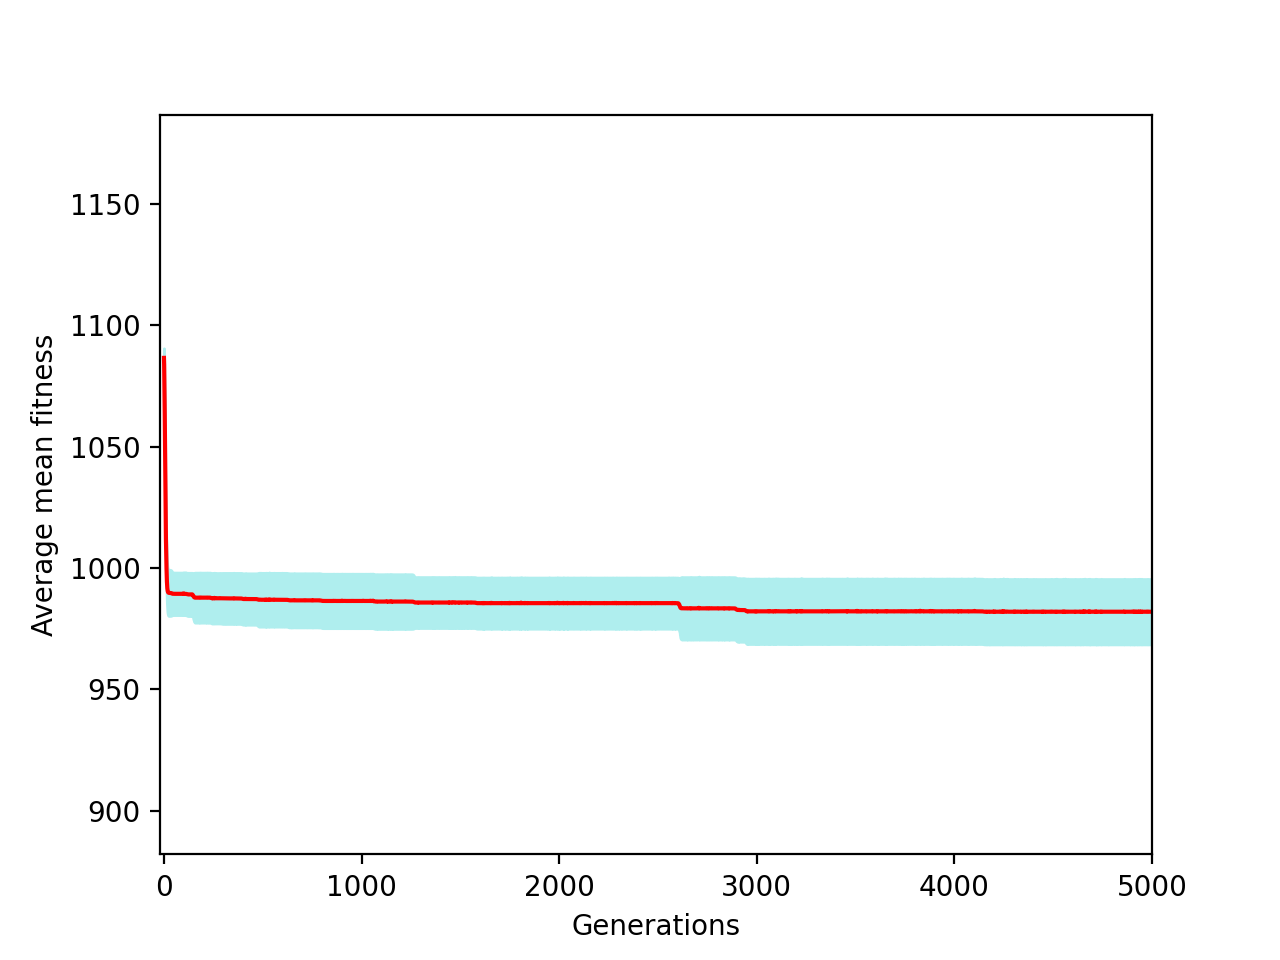
\includegraphics[scale=0.35]{E-n51-k5-mean}
    \caption{E-n51-k5}
    \label{fig:my_label}
\end{figure}

\begin{figure}[h!]
    \centering
    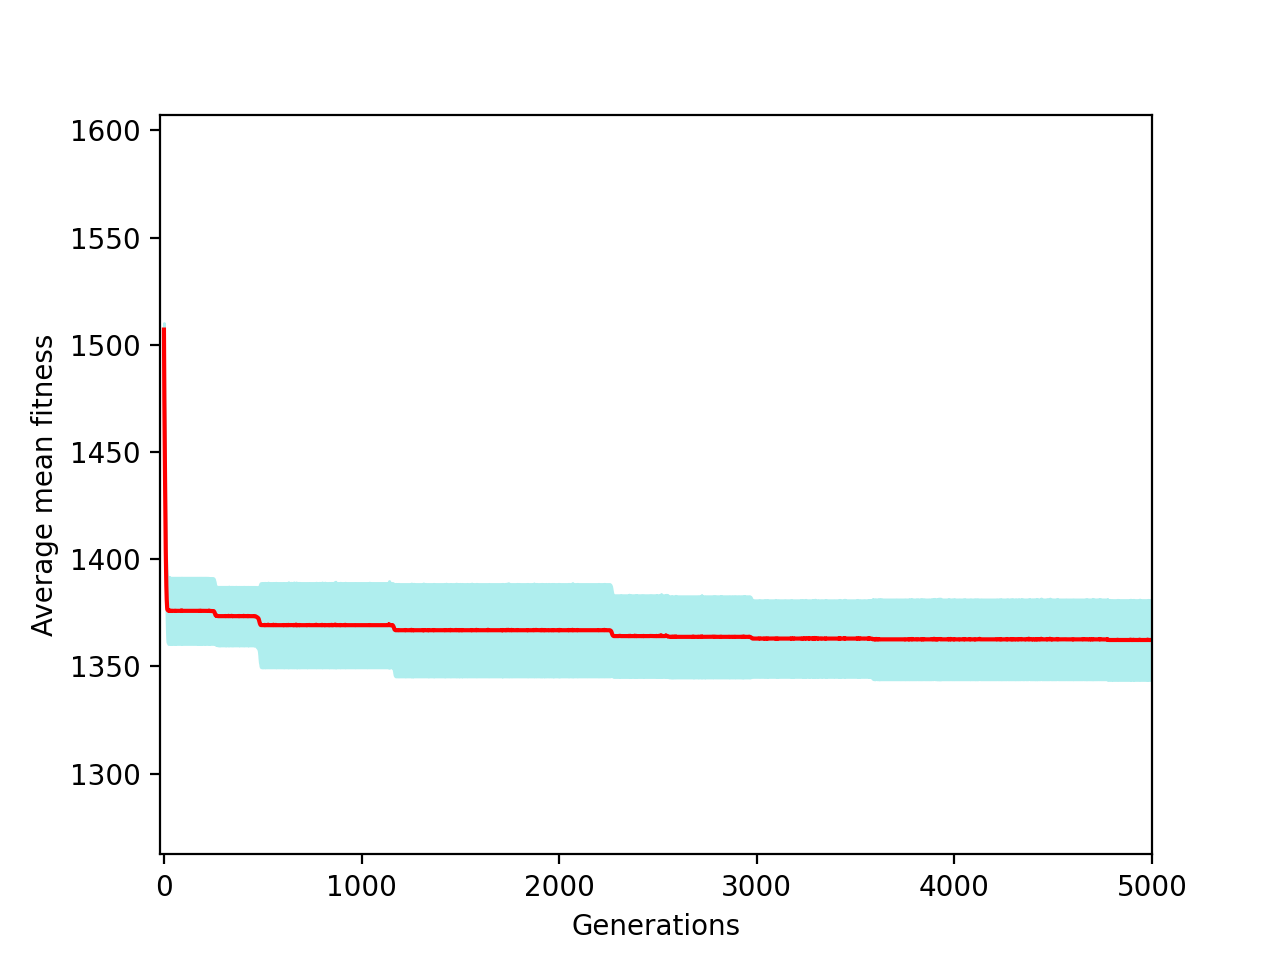
\includegraphics[scale=0.35]{E-n76-k7-mean}
    \caption{E-n76-k7}
    \label{fig:my_label}
\end{figure}


\begin{figure}[h!]
    \centering
    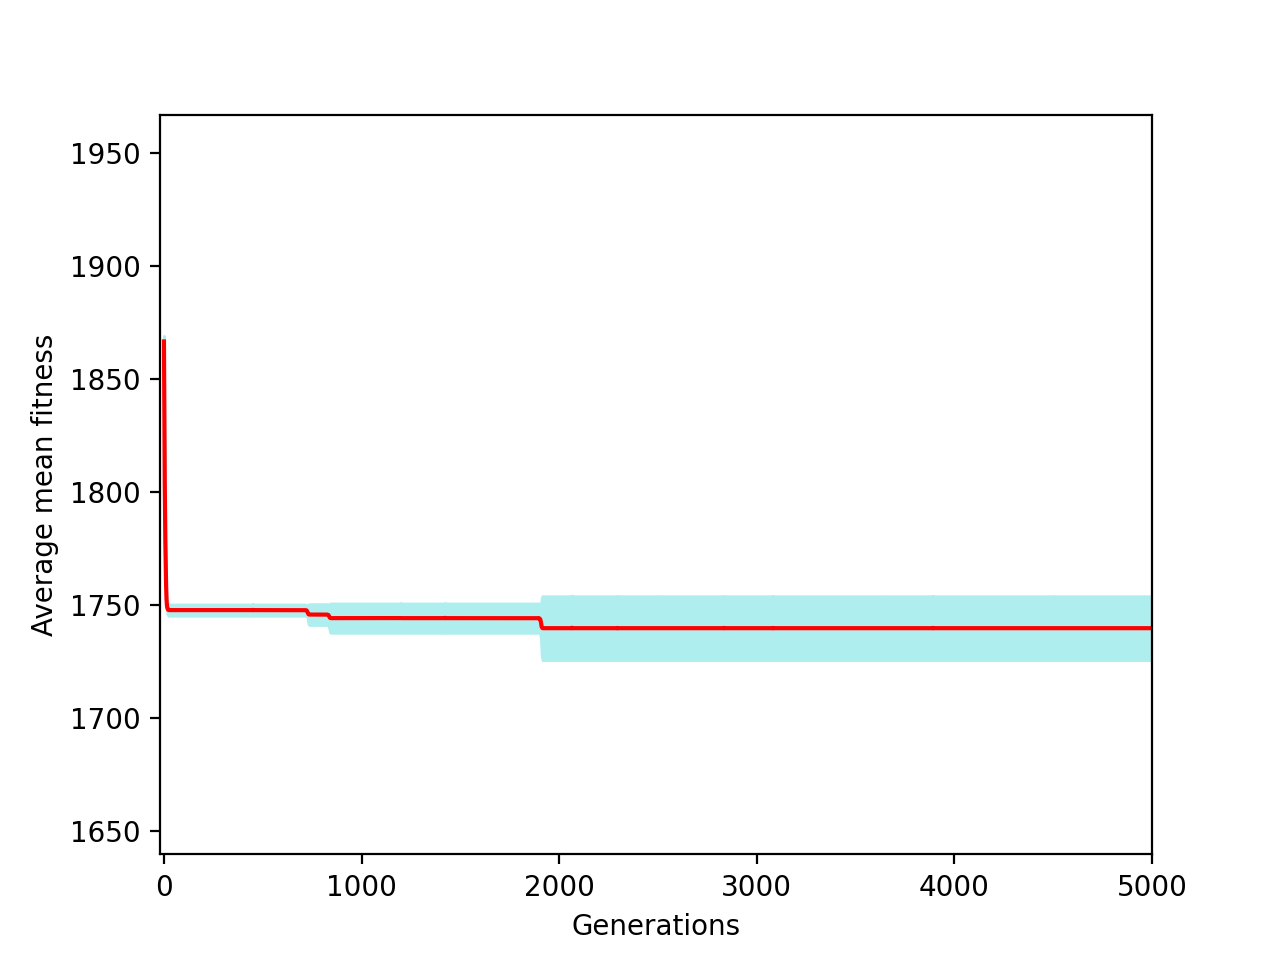
\includegraphics[scale=0.35]{E-n101-k8-mean}
    \caption{E-n101-k8}
    \label{fig:my_label}
\end{figure}


\begin{figure}[h!]
    \centering
    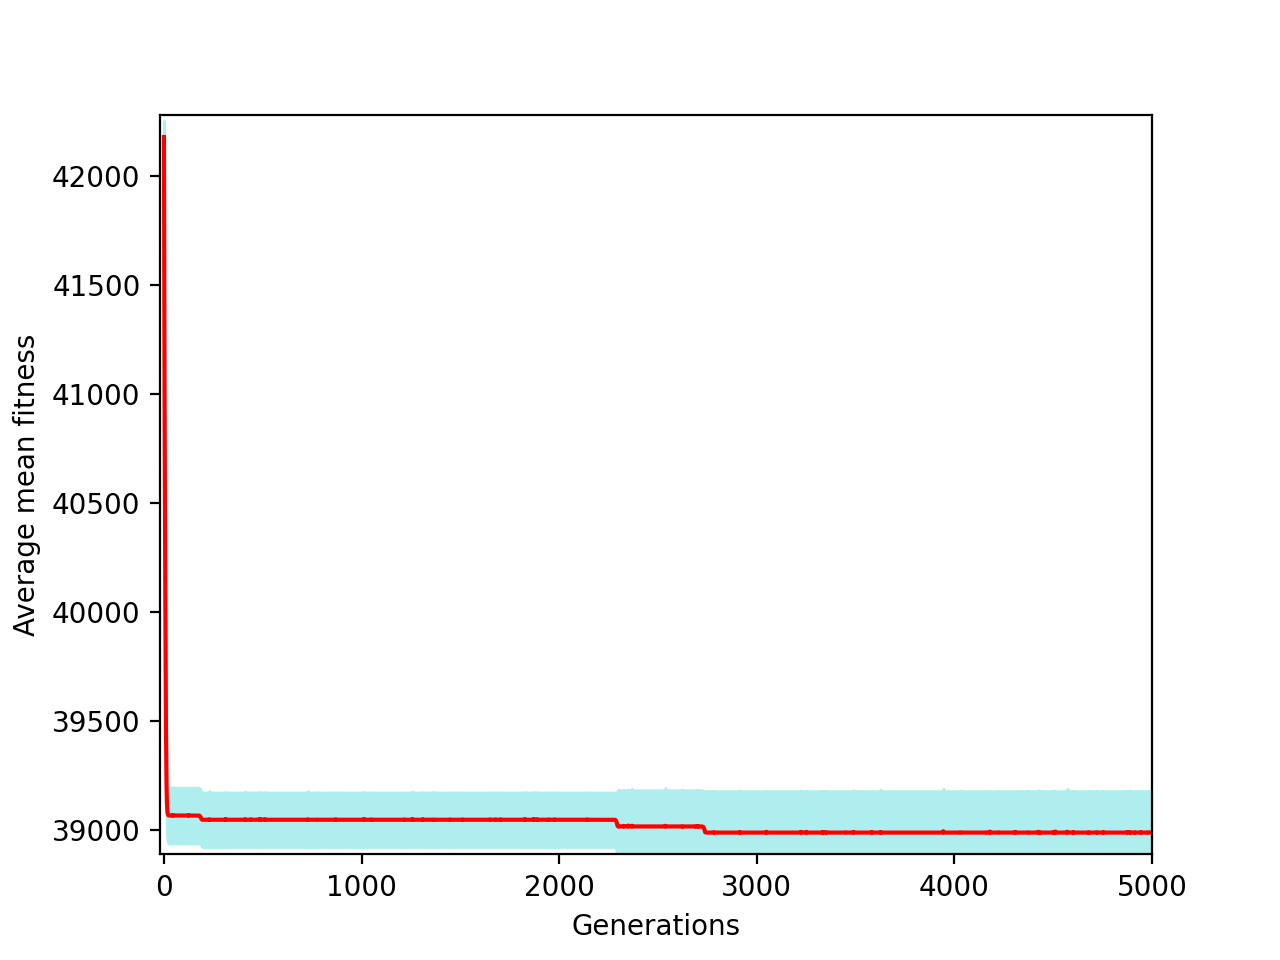
\includegraphics[scale=0.35]{X-n143-k7-mean}
    \caption{X-n143-k7}
    \label{fig:my_label}
\end{figure}
\newpage

In addition to Genetic Algorithm, we also propose \textit{Google OR-Tools} \cite{ortools} to handle the EVRP. Google OR-Tools provides us a tool to handle combinatorial optimization problem (C.O.P) via an open-source software. This tool can help us to find the best (or relatively good) solution for our present problem through a large set of possible feasible solutions.\\


In the vehicle routing problem, Google OR-Tools is designed to find the optimal routes as the solution, and OR-Tools defines an optimal route as the route with the smallest total distance and all constraints are satisfied \cite{vrp_demonstration}. Since OR-Tools has not introduced an obvious tool to solve the EVRP but the VRP only, we shall demonstrate our approach to make OR-Tools able to solve this problem effectively.

\section{Results}
This section is to show the result of the EVRP when applying GA. Besides, we also compare our result with Google OR-Tools and the winner in \textit{CEC-12 Competition on Electric Vehicle Routing Problem}\footnote{https://mavrovouniotis.github.io/EVRPcompetition2020}.
\subsection*{Settings}
In this work, we choose the population size as 400 and number of generation as 5000 for Genetic Algorithm.\\

Google OR-Tools is a restricted framework and there is few documents to reference which leads to many a difficulty when applying this framework into solving the EVRP. When applying OR-Tools to solve this problem, we got into trouble which is EVs forgot to pay energy cost while moving to another recharging stations but still got fully recharged. This unfortunately leads to the OR-Tools can not give any appropriate solutions.\\

Hence, we came into decision to restrict EVs' battery level to a range calculated by:
\begin{equation}
    Q = Q - max{\sum_{i \in V}{\left(min{\sum_{j\in R, i \neq j}{\rho d_{ij}x_{ij}}}\right)}}
\end{equation}

This helps us to find the feasible solution for some initial instances, but none for later instances.
\subsection*{Test instances}
Our benchmark set for this paper comes from the \textit{CEC-12 Competition on Electric Vehicle Routing Problem} \cite{evrp_benchmark}.
\subsection*{Table of results}
There are 17 instances in the standard benchmark, we just show solvable ones however. There are 3 tables in total, which are GA's results (Table 1), Google OR-Tools' results (Table 2) and the winner team in the competition's one (Table 3). Each table is demonstrated as: the first column consists of name of instances; the second, third, fourth and the last one respectively consists of mean, max, min and standard deviation results in 10 runs.\\
We also give out 8 plots responding to 8 first instances solve by GA. The x-axis stands for number of generations and the y-axis is the average best fitness in 10 runs. The pale turquoise zone represents for the standard deviation.

\subsection*{Result analysis}
Incomplete as Google OR-Tools is, it still gives out the solution for the first five instances, in which the results for E-n22-k4 and E-n51-k5 is excellent; the results are even better than our GA's and quite close to the winner team's results.\\

Our GA's result in Table 3 is outstanding with n < 50 and it is quite close to the winner team's results. It becomes worse or even unsolvable, however, when n $>$ 50 and n $>$ 200, respectively.\\

When observing plots, it is clear that K-means helps Genetic algorithm to generate a relatively good population. This can be shown since the green line has a tendency to decrease, which is a good signal. Thus, if we increase number of generations, that green line has a probability to go shallower. However, crossover as soon as the loop starts makes GA unable to keep good individuals in the generating step. This is the reason for green line goes up when starting and go downhill when the numbers of generation increase in some plot.
\begin{table}[h!]
\centering
\begin{tabular}{|c|c|c|c|c|c|c|c|c|c|c|c|c|c|}
     \hline 
     Instances & mean & max & min & stdev \\
     \hline
     E-n22-k4 & 401 & 401 & 401 & 0\\
     \hline
     E-n23-k3 & 701&701 & 701&0 \\
    \hline
     E-n30-k3 & 635.4 & 644 & 603 & 11.7149\\
     \hline
     E-n33-k4 & 997.8 & 1012 & 967 & 19.3845\\
     \hline
     E-n51-k5 & 606.8&624 & 572&14.4069 \\
    \hline
\end{tabular}

% \captionsetup{justification=centering}
\caption{Google OR-Tools' results}
\end{table}

\begin{table}[h!]
    \centering
\begin{tabular}{|c|c|c|c|c|c|c|c|c|c|c|c|c|c|}
     \hline 
     Instances & mean & max & min & stdev \\
     \hline
     E-n22-k4 & 384.67 & 384.67 & 384.67 & 0\\
     \hline
     E-n23-k3 & 571.94 & 571.94 &571.94 &0 \\
    \hline
     E-n30-k3 & 509.47 & 509.47 & 509.47 & 0\\
     \hline
     E-n33-k4 & 840.14 & 840.46 & 840.43 & 1.18\\
     \hline
     E-n51-k5 & 529.90 & 548.98 & 543.26 & 3.52\\
    \hline
    E-n76-k7 & 692.94 & 707.49 & 697.89 & 3.09\\
    \hline
    E-n101-k8 & 839.29 & 853.34&853.34 &4.73 \\
    \hline
    X-n143-k7 &16028.05 &16883.38 &16459.31 & 242.59\\
    \hline
\end{tabular}
    \caption{Variable Neighborhood Search’s results by D. Woller, V. Vavra, V. Kozak, M. Kulich}
    \label{tab:my_label}
\end{table}

\begin{table}[h!]
    \centering
        \begin{tabular}{|c|c|c|c|c|c|c|c|}
    \hline
         Instances & mean & max & min & stdev  \\
         \hline 
         E-n22-k4&	424.95&	464.39&	402.53&	18.7183\\
         \hline
E-n23-k3	&632.19&	671.62&	607.01&	23.5857\\
\hline
E-n30-k3	&633.81	&669.65&	593.78&	29.0584\\
\hline
E-n33-k4&	938.66&	959.64	&898.62&	19.4428\\
\hline
E-n51-k5&	981.97&	1004.74&	961.03&	14.1877\\
\hline
E-n76-k7&	1362.30&	1391.84&	1323.60&	19.6518\\
\hline
E-n101-k8&	1739.82&	1752.73&	1702.07&	14.9056\\
\hline
X-n143-k7 &	38987.96 &	39384.5 &	38683.4	 & 200.2779\\\hline
    \end{tabular}
    \caption{Genetic Algorithm's results}
    \label{tab:my_label}
\end{table}
\section{Future work}
In this paper, due to the time pressure, we did not do the mutation. However, we do believe that mutation step is a crucial factor in GA and it might increase the quality of our solution. We will research it more in the future.\\

We also research a better heuristic function for locating recharging stations compared to our present one. This is due to the fact that adding recharging stations based on the energy cost from the next node to the nearest recharging station of that node is not good at all. We could choose a further recharging station sharing the same direction to the solution's trajectory, as long as going to that recharging station does not exhaust the whole remaining energy level.\\

Besides, we would also research more efficient crossover methods. We just solve the EVRP with the problem size of less than 200 in present, the population with a larger than 200 problems size is unacceptable poor since there is no feasible solution in the indigenous population. Thus, we will also find a more effective way to initialize the starting population as good as possible to solve large-scale problems and improve the smaller-problem size solution.

\section{Conclusion}
In this work, we consider the Electric Vehicle Routing Problem. We did propose a potential solution with several techniques, e.g. Genetic Algorithm, Dijkstra, K-means and some heuristics.\\

Separating a big problem into two smaller ones, which are electric vehicle routing and locations of charging stations, enables us inheriting results from previous researches in GA for the VRP. Then, we could design an additional heuristic to add recharging stations into chromosomes to solve the EVRP.\\

However, heuristics seem to be insufficient despite sustaining feasible at least one solution. Furthermore, generating a not so well population prevents GA from finding any solution. Thus, beside the proposed solution - which is K-means, we would find newer methods.

% regular IEEE prefers the singular form
\section*{Acknowledgment}
The authors would like to thank the support of the Evolutionary Learning and Optimization (ELO@UIT) group at the University of Information Technology, Vietnam National University HCMC.
\newpage
\section*{Biography}
\subsection*{An Vo}

\begin{figure}[h!]
    \centering
    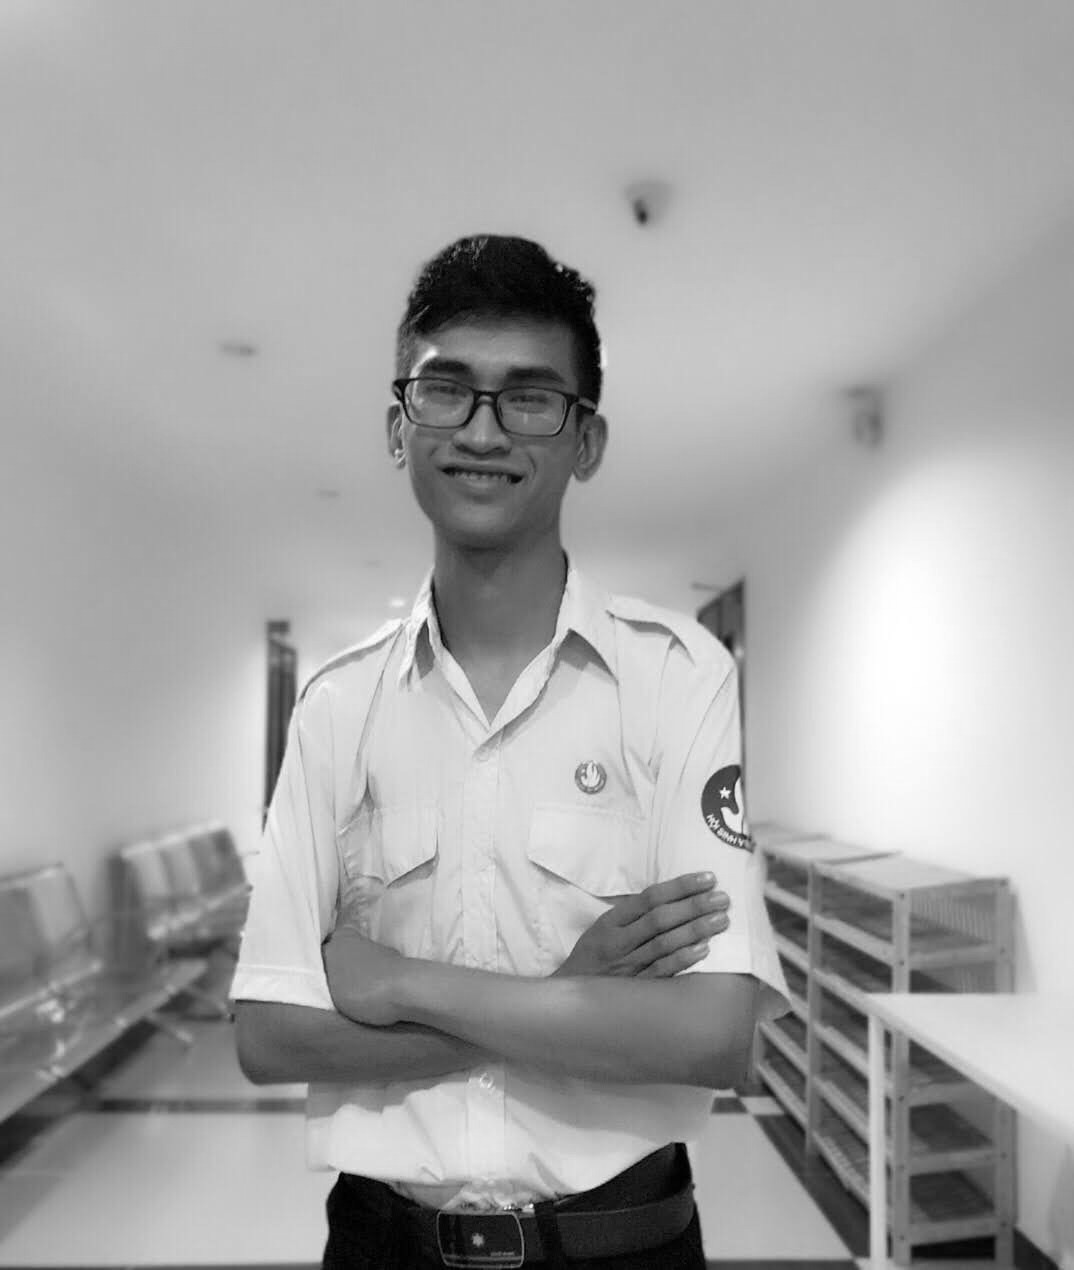
\includegraphics[scale=0.1]{AV}
    \label{fig:my_label}
\end{figure}
An Vo graduated in 2019 at Phan Ngoc Hien High school for the gifted, Ca Mau province, specified for Mathematics - Informatics. From 2019, he has been studying at University of Information Technology, Vietnam National University HCMC, faculty of Computer Science, class of KHCL2019.1.\\

He received several prizes at provincial, Southern and National Olympics in Informatics. Besides, he has also achieved himself three scholarships from Office of Student Affairs, UIT - VNU HCM and two scholarships from Office of Excellent Programs, UIT - VNU HCM.

\subsection*{Tan Ngoc Pham}
\begin{figure}[h!]
    \centering
    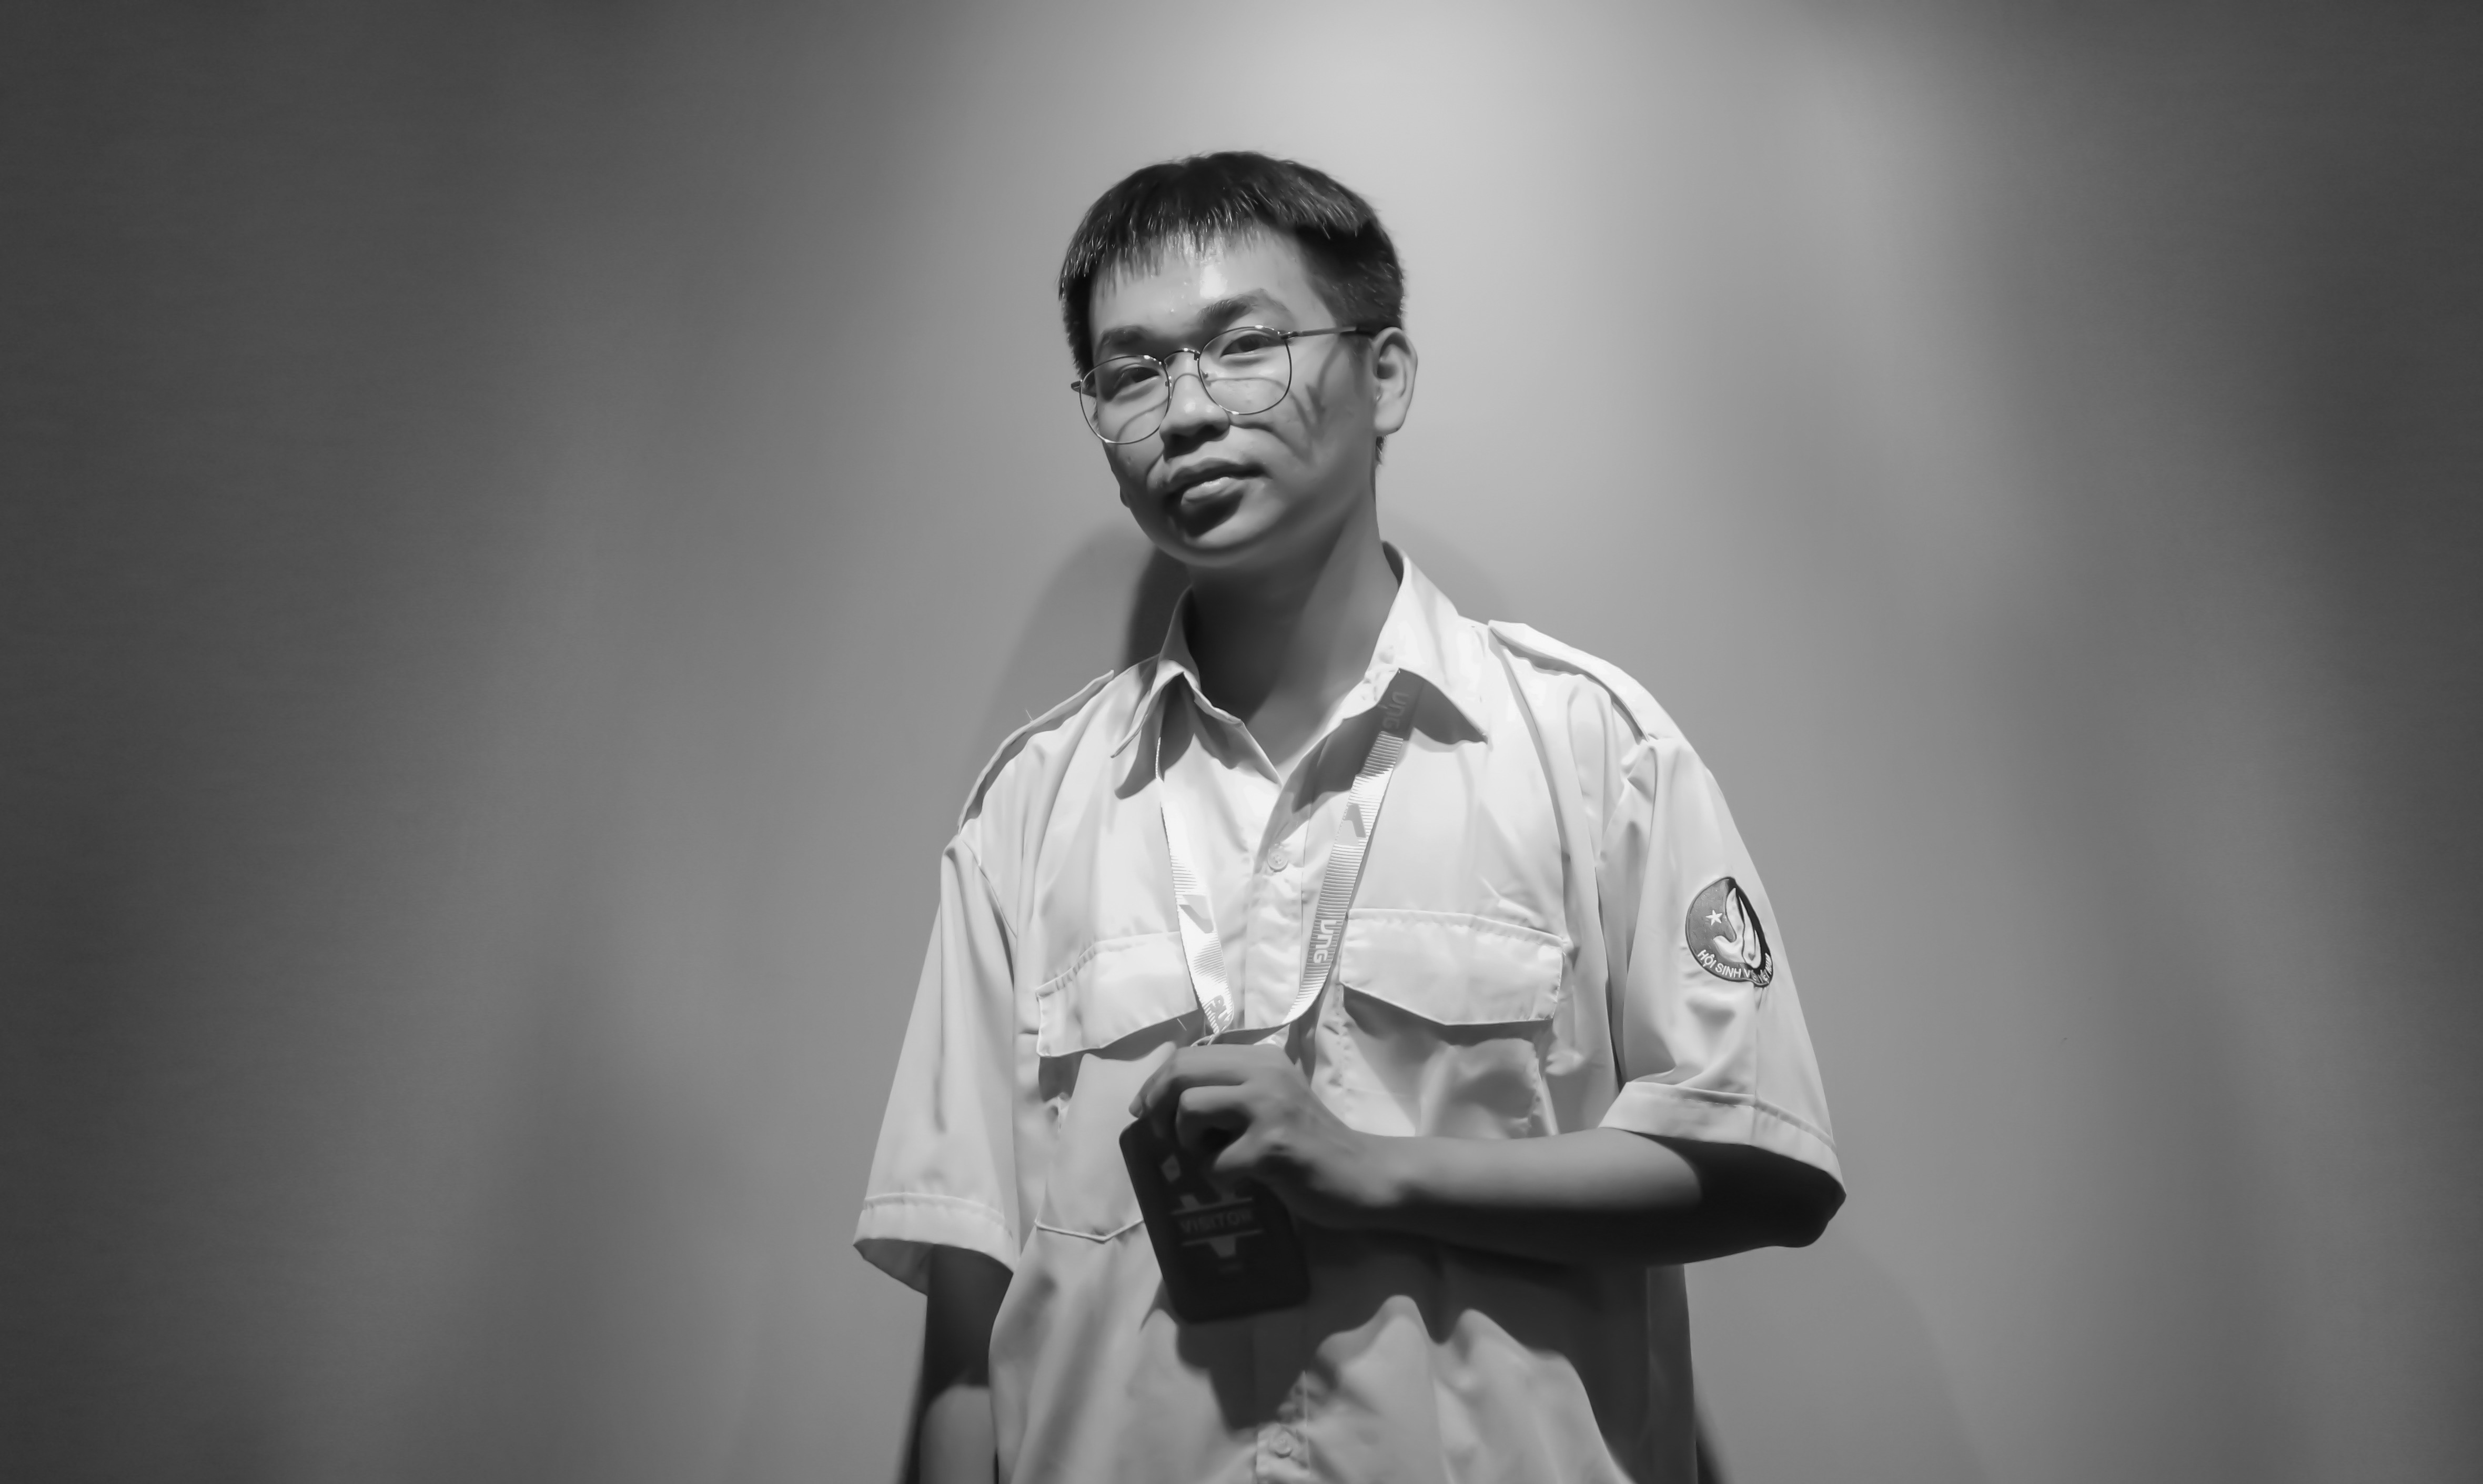
\includegraphics[scale=0.03]{NT}
    \label{fig:my_label}
\end{figure} 
Tan Ngoc Pham graduated in 2019 at Nguyen Du High school for the gifted, Dak Lak province, specified for English. From 2019, he has been studying at University of Information Technology, Vietnam National University HCMC, faculty of Computer Science, class of KHCL2019.2.\\

He received several prizes at provincial and National Olympics in English and second prize in the National Olympics in English is among the top prizes of him.

% An example of a floating figure using the graphicx package.
% Note that \label must occur AFTER (or within) \caption.
% For figures, \caption should occur after the \includegraphics.
% Note that IEEEtran v1.7 and later has special internal code that
% is designed to preserve the operation of \label within \caption
% even when the captionsoff option is in effect. However, because
% of issues like this, it may be the safest practice to put all your
% \label just after \caption rather than within \caption{}.
%
% Reminder: the "draftcls" or "draftclsnofoot", not "draft", class
% option should be used if it is desired that the figures are to be
% displayed while in draft mode.
%
%\begin{figure}[!t]
%\centering
%\includegraphics[width=2.5in]{myfigure}
% where an .eps filename suffix will be assumed under latex, 
% and a .pdf suffix will be assumed for pdflatex; or what has been declared
% via \DeclareGraphicsExtensions.
%\caption{Simulation results for the network.}
%\label{fig_sim}
%\end{figure}

% Note that the IEEE typically puts floats only at the top, even when this
% results in a large percentage of a column being occupied by floats.


% An example of a double column floating figure using two subfigures.
% (The subfig.sty package must be loaded for this to work.)
% The subfigure \label commands are set within each subfloat command,
% and the \label for the overall figure must come after \caption.
% \hfil is used as a separator to get equal spacing.
% Watch out that the combined width of all the subfigures on a 
% line do not exceed the text width or a line break will occur.
%
%\begin{figure*}[!t]
%\centering
%\subfloat[Case I]{
\includegraphics[width=2.5in]{box}%
%\label{fig_first_case}}
%\hfil
%\subfloat[Case II]{
\includegraphics[width=2.5in]{box}%
%\label{fig_second_case}}
%\caption{Simulation results for the network.}
%\label{fig_sim}
%\end{figure*}
%
% Note that often IEEE papers with subfigures do not employ subfigure
% captions (using the optional argument to \subfloat[]), but instead will
% reference/describe all of them (a), (b), etc., within the main caption.
% Be aware that for subfig.sty to generate the (a), (b), etc., subfigure
% labels, the optional argument to \subfloat must be present. If a
% subcaption is not desired, just leave its contents blank,
% e.g., \subfloat[].


% An example of a floating table. Note that, for IEEE style tables, the
% \caption command should come BEFORE the table and, given that table
% captions serve much like titles, are usually capitalized except for words
% such as a, an, and, as, at, but, by, for, in, nor, of, on, or, the, to
% and up, which are usually not capitalized unless they are the first or
% last word of the caption. Table text will default to \footnotesize as
% the IEEE normally uses this smaller font for tables.
% The \label must come after \caption as always.
%
%\begin{table}[!t]
%% increase table row spacing, adjust to taste
%\renewcommand{\arraystretch}{1.3}
% if using array.sty, it might be a good idea to tweak the value of
% \extrarowheight as needed to properly center the text within the cells
%\caption{An Example of a Table}
%\label{table_example}
%\centering
%% Some packages, such as MDW tools, offer better commands for making tables
%% than the plain LaTeX2e tabular which is used here.
%\begin{tabular}{|c||c|}
%\hline
%One & Two\\
%\hline
%Three & Four\\
%\hline
%\end{tabular}
%\end{table}


% Note that the IEEE does not put floats in the very first column
% - or typically anywhere on the first page for that matter. Also,
% in-text middle ("here") positioning is typically not used, but it
% is allowed and encouraged for Computer Society conferences (but
% not Computer Society journals). Most IEEE journals/conferences use
% top floats exclusively. 
% Note that, LaTeX2e, unlike IEEE journals/conferences, places
% footnotes above bottom floats. This can be corrected via the
% \fnbelowfloat command of the stfloats package.


% trigger a \newpage just before the given reference
% number - used to balance the columns on the last page
% adjust value as needed - may need to be readjusted if
% the document is modified later
%\IEEEtriggeratref{8}
% The "triggered" command can be changed if desired:
%\IEEEtriggercmd{\enlargethispage{-5in}}


\bibliographystyle{IEEEtran}
\bibliography{ref.bib}


% that's all folks
\end{document}


